\documentclass[12pt,fleqn,a4paper]{report}
\usepackage[many]{tcolorbox}
\usepackage{times}
\usepackage[utf8]{inputenc}
\usepackage[T1]{fontenc}
\usepackage[french]{babel}
\usepackage{array,multirow,makecell}
\setcellgapes{1pt}
\makegapedcells
\newcommand{\chaptertoc}[1]{\chapter*{#1}
\addcontentsline{toc}{chapter}{#1}
\markboth{{#1}}{{#1}}}
\usepackage{amsmath}
\usepackage{amssymb}
\usepackage{rotating}
\usepackage{lscape}
\usepackage{amsthm}
\usepackage{makeidx}
\usepackage{listings}
\usepackage{fancybox}
\usepackage{pifont}
\usepackage{hyperref}
\usepackage[table,xcdraw]{xcolor}
\usepackage[normalem]{ulem}
\useunder{\uline}{\ul}{}
\usepackage{ragged2e}

% ====== BIBLIOGRAPHY: biblatex ONLY (supprime natbib) ======
\usepackage[style=numeric,backend=biber]{biblatex}
\addbibresource{bbbib.bib}
% ===========================================================

\definecolor{main}{HTML}{5989cf}
\definecolor{sub}{HTML}{cde4ff}
\makeatletter
\newcommand\blankpage{%
    \null
    \thispagestyle{empty}%
    \addtocounter{page}{-1}%
    \newpage}
\makeatother
\tcbset{
    sharp corners,
    colback = white,
    before skip = 0.2cm,
    after skip = 0.5cm
}
\newtcolorbox{boxI}{
    colback = sub,
    colframe = main,
    boxrule = 0pt,
    toprule = 6pt
}

\usepackage{titlesec}
\titleformat{\chapter}[display]
{\normalfont\huge\bfseries}{\chaptertitlename\ \thechapter}{20pt}{\Huge}

\usepackage{fancyhdr}
\usepackage{epsfig}
\usepackage{epstopdf}
\usepackage{subfig}
\usepackage{multirow}
\usepackage{algorithm}
\usepackage{algorithmic}
\usepackage[francais]{minitoc}
\mtcselectlanguage{french}
\setcounter{minitocdepth}{1}
\usepackage{graphicx}
% Tous les fichiers images (logos + diagrammes) sont cherches automatiquement
% dans ces trois dossiers : plus besoin de prefixer chaque \includegraphics.
\graphicspath{{Image/}{images/}{rapport_diagrams/}}
\usepackage{tabularx}
\usepackage{booktabs}
\usepackage{fancyvrb}
\setcounter{secnumdepth}{4}
\setcounter{tocdepth}{4}
\usepackage{latexsym}
\usepackage{calc}
\usepackage{lettrine}
\usepackage{a4wide}
\usepackage{verbatim}
\usepackage{moreverb}
\usepackage{pdfpages}
\usepackage{float}
\usepackage{caption}
\usepackage{longtable}
\captionsetup{position=below}
\newcolumntype{R}[1]{>{\raggedleft\arraybackslash }b{#1}}
\newcolumntype{L}[1]{>{\raggedright\arraybackslash }b{#1}}
\newcolumntype{C}[1]{>{\centering\arraybackslash }b{#1}}
\renewcommand{\baselinestretch}{1.1}
\setlength{\parskip}{0.3cm}
\usepackage{color}

\usepackage[Lenny]{fncychap}
\ChTitleVar{\Huge\sffamily\bfseries}

\newtheorem{Theorem}{Theorem}[chapter]
\newtheorem{Example}{Example}[chapter]
\newtheorem{c-Example}{Counter-example}[chapter]
\newtheorem{Proposition}{Proposition}[chapter]
\newtheorem{Definition}{Definition}[chapter]
\newtheorem{Lemma}{Lemma}[chapter]
\newtheorem{Corol}{Corollary}[chapter]

\vfuzz2pt
\hfuzz2pt

\colorlet{LightRubineRed}{red!70!}
\colorlet{Mycolor1}{blue!40!black!60!}

\pagestyle{fancy}
\fancyhead[LO,RE]{\textsl{\rightmark}}
\renewcommand{\headrulewidth}{0.4pt}
\renewcommand{\chaptermark}[1]%
{\markboth{\itshape{Chapter~\thechapter~: \ #1}}{}}
\renewcommand{\sectionmark}[1]%
{\markright{\itshape{Section~\thesection~--~\ #1}}}
\lhead[\thepage]{\leftmark}
\rhead[\leftmark]{\thepage}

\begin{document}
\dominitoc
\justifying
\begin{justify}

\thispagestyle{empty}
\begin{figure}[]
\begin{minipage}[l]{.3\textwidth}
\begin{center}
\flushleft \includegraphics[width=3cm]{univK.jpg}
\end{center}
\end{minipage}
\begin{minipage}{.36\textwidth}
\begin{center}
\footnotesize{République Tunisienne
Ministère de l'Enseignement Supérieur, de
la Recherche Scientifique et de la
Technologie }
\noindent
{\color{Mycolor1} \rule{\linewidth}{0.5mm} }
\footnotesize{Université de Kairouan
Institut Supérieur d'Informatique et de
Gestion de Kairouan }
\end{center}
\end{minipage}
\begin{minipage}{.32\textwidth}
\begin{center}
\flushright 
\includegraphics[width=4cm]{isigk.png}
\end{center}
\end{minipage}
\end{figure}

\begin{center}
\textcolor{white}{ }
\noindent
{\color{Mycolor1} \rule{\linewidth}{0.5mm} }\\
\Large{\textbf{ \textit{PROJET }}} \\
\bigskip
{\color{Mycolor1} \rule{\linewidth}{1mm} }\\
{\huge \textbf{Application de Livraison}} \\
\noindent
{\color{Mycolor1} \rule{\linewidth}{1mm} }

\Large{Élaboré par: \textit{Adam Cherif}}\\
\end{center}

\large{\textbf{Encadreur Académique: Mme Olfa Harrabi}}\\
\noindent
{\color{Mycolor1} \rule{\linewidth}{0.5mm} }
\begin{center}
Année universitaire : 2025 / 2026
\end{center}

\tableofcontents
\newpage

\thispagestyle{empty}

\vspace*{2cm}

\begin{center}
  \rule[0.5ex]{3.2cm}{0.5pt} \quad {\Huge \textbf{Remerciements}} \quad \rule[0.5ex]{3.2cm}{0.5pt}
\end{center}

\vspace{1.5cm}

\noindent \textbf{M}es remerciements s'adressent tout d'abord au bon Dieu le tout puissant et miséricordieux, qui m'a donné la force, la volonté et la patience pour accomplir ce modeste travail.

\vspace{0.8cm}

\noindent \textbf{J}e tiens à exprimer ma profonde gratitude et mes sincères remerciements à mon encadreuse académique, \textbf{Mme Olfa Harrabi}, pour son encadrement précieux, ses conseils avisés et sa disponibilité tout au long de la réalisation de ce projet.

\vspace{0.8cm}

\noindent \textbf{M}es remerciements s'adressent également aux membres du jury d'avoir accepté d'évaluer ce travail, ainsi qu'à l'ensemble du corps professoral de l'\textbf{Institut Supérieur d'Informatique et de Gestion de Kairouan (ISIGK)}.
\newpage
\thispagestyle{empty}

\vspace*{1.5cm}

\begin{center}
  \rule[0.5ex]{3.2cm}{0.5pt} \quad {\Huge \textbf{Dédicaces}} \quad \rule[0.5ex]{3.2cm}{0.5pt}
\end{center}

\vspace{1.2cm}

\begin{center}
  \noindent \textbf{À} mes chers parents, pour leurs sacrifices inestimables, leur soutien inconditionnel, leurs prières quotidiennes et leur amour infini qui ont éclairé mon parcours.

  \vspace{0.7cm}

  \noindent \textbf{À} mon cher frère, mon compagnon de route, mon guide et ma fierté, que Dieu le garde en bonne santé.

  \vspace{0.7cm}

  \noindent \textbf{À} toute mes proches, pour leurs encouragements constants et leur présence bienveillante à chaque étape.



  \vspace{0.7cm}

  \noindent \textbf{À} moi-même, en reconnaissance de la patience, de la persévérance, de la passion et des efforts soutenus investis dans la réalisation de ce projet, malgré les défis et les nuits de labeur.

  \vspace{1.1cm}

  \noindent \textbf{Q}u'ils trouvent tous dans ce modeste travail le témoignage de ma profonde affection, de mon attachement indéfectible et le fruit d'une grande détermination.
\end{center}

\newpage

\newpage
\chapter*{\hfill Introduction générale \hfill}
\markboth{\small{Introduction générale}}{\small{Introduction générale}}
\addcontentsline{toc}{chapter}{Introduction générale}

\renewcommand{\thepage}{\arabic{page}}
\setcounter{page}{1}

Avec l'évolution rapide des technologies numériques et la généralisation de l'utilisation des smartphones, les applications de livraison sont devenues un service essentiel dans la vie quotidienne. Elles permettent aux utilisateurs de commander facilement des produits, des repas ou d'envoyer des colis, tout en offrant aux commerçants et aux livreurs une plateforme efficace pour gérer leurs activités.

Dans ce contexte, les plateformes de livraison jouent un rôle important dans la simplification du processus de commande et de distribution. Elles permettent de connecter différents acteurs tels que les clients, les commerçants et les livreurs au sein d'un même système numérique, facilitant ainsi la gestion des commandes, le suivi des livraisons et la communication entre les utilisateurs.

Le présent projet consiste à concevoir et développer une application de livraison permettant aux clients de commander des plats ou des produits, ainsi que d'envoyer des colis à travers une interface simple et intuitive. L'application permet également aux commerçants de gérer leurs produits et leurs plats, tandis que les livreurs peuvent recevoir et effectuer les livraisons assignées par le système.

L'objectif principal de cette application est d'optimiser le processus de commande et de livraison en proposant une solution numérique efficace qui améliore l'expérience utilisateur, facilite la gestion des commandes et assure un suivi en temps réel des livraisons.

\vspace{2cm}

%************CHAP1***********
\chapter{Problématique et Analyse des Besoins}

\section{Contexte et enjeux du projet :}

Le paysage de la consommation en Tunisie vit actuellement une mutation majeure, accélérée par l'usage quotidien des téléphones intelligents et le besoin de rapidité des citoyens. Aujourd'hui, commander un repas ou acheter des produits de première nécessité sans se déplacer est devenu une habitude pour de nombreux Tunisiens. Ce projet se place au cœur de cette révolution numérique en proposant une solution moderne qui répond aux besoins réels du marché local.  L'initiative débute par une phase pilote stratégique dans le gouvernorat de Kairouan. Ce choix permet de tester l'efficacité du service dans une zone dynamique avant de déployer l'application sur tout le territoire tunisien. L'ambition est de créer un réseau national capable de relier efficacement les clients et les commerçants.  L'enjeu principal de ce travail est de regrouper, au sein d'une seule et même interface, des services qui sont habituellement dispersés. La plateforme permet non seulement de commander auprès de restaurants ou de supermarchés, mais elle innove également en intégrant le transport de colis entre particuliers (P2P) et la gestion simplifiée du paiement de factures.  Enfin, au-delà de l'aspect pratique pour l'utilisateur, ce projet accorde une importance capitale aux partenaires commerciaux.
\newpage
\section{Etude de l'existant :}
L'analyse des solutions actuelles constitue une phase primordiale dans le cycle de développement de notre projet. En effet, elle offre l'opportunité d'évaluer les systèmes en place dans le but d'innover en créant une nouvelle plateforme ou d'optimiser une offre déjà établie. Face à la multitude d'applications dédiées aux services de livraison sur le marché, notre démarche s'est orientée vers l'examen des plateformes les plus influentes, tant à l'échelle locale qu'internationale
\subsection{Analyse de l'existant :}


Nous pouvons classer les applications de livraison selon les services qu'elles proposent :\\
\vspace{0.3cm}
\textbf{Yassir Express :} Une application  qui permet de livrer des repas préparés, des produits cosmétiques ainsi que des fruits et légumes .
\begin{figure}[H]
    \centering
    \fbox{\includegraphics[width=0.55\textwidth,keepaspectratio]{Interface de yassir 1.png}}
    \caption{Captures d'écran de l'application Yassir Express}
\end{figure}

\textbf{Livrina:} Lvrina est une solution mobile tout-en-un qui regroupe la commande de repas, les achats du quotidien et la gestion des factures. En intégrant un système d'envoi de colis entre particuliers, la plateforme simplifie la logistique de proximité et optimise le quotidien de ses utilisateurs.\\
\begin{figure}[H]
    \centering
    \fbox{\includegraphics[width=0.55\textwidth,keepaspectratio]{interface de Livrina.png}}
    \caption{Captures d'écran de l'application Livrina}
\end{figure}
\subsubsection{Livraison de repas et de produits de première nécessité :}
Ces applications se concentrent principalement sur le transport d'aliments et d'achats quotidiens.

\begin{itemize}
    \item \textbf{Glovo :} plateforme internationale de livraison multi-services permettant de commander des repas, d'effectuer des achats du quotidien et d'expédier de petits colis en zone urbaine.
    \item \textbf{KooL :} application tunisienne dédiée à la livraison de repas à domicile, proposant la commande en ligne auprès de restaurants locaux et un suivi de commande en temps réel.
    \item \textbf{ZigZag Delivery :} solution tunisienne spécialisée dans la commande et la livraison rapide de repas, reliant les consommateurs aux restaurants locaux avec un suivi.
\end{itemize}

\section{Critique de l'existant}

L'analyse des solutions de livraison en Tunisie (\textit{Glovo, Yassir Express, KooL, ZigZag Delivery, Livrina}) montre que ces plateformes restent principalement concentrées dans les grandes métropoles. Bien qu'elles répondent à certains besoins, elles présentent des limites importantes. Cette section propose une étude détaillée des forces et des faiblesses de chaque concurrent, suivie d'une analyse thématique et d'un tableau comparatif.

\subsection{Analyse détaillée des acteurs du marché}

% ==================== GLOVO ====================
\subsubsection*{\Large \textbf{1. Glovo}}
\vspace{0.2cm}

\noindent \textbf{\underline{Points forts :}}
Interface moderne et simple à utiliser, large gamme de catégories (repas, courses, pharmacie) et forte notoriété internationale.

\vspace{0.2cm}
\noindent \textbf{\underline{Limites et critiques :}}
\begin{itemize}
    \item \textbf{Absence totale à Kairouan :} Le service cible uniquement Tunis et les grandes villes côtières, délaissant les gouvernorats de l'Intérieur.
    \item \textbf{Commissions élevées :} Les taux prélevés aux commerçants partenaires (entre 20\% et 30\%) réduisent fortement leurs marges.
    \item \textbf{Rigidité de la plateforme :} Faible capacité à s'adapter aux besoins spécifiques des villes secondaires.
\end{itemize}

\vspace{0.5cm}

% ==================== YASSIR EXPRESS ====================
\subsubsection*{\Large \textbf{2. Yassir Express}}
\vspace{0.2cm}

\noindent \textbf{\underline{Points forts :}}
Écosystème régional intégrant transport et livraison, appuyé par une bonne infrastructure technique.

\vspace{0.2cm}
\noindent \textbf{\underline{Limites et critiques :}}
\begin{itemize}
    \item \textbf{Couverture quasi-inexistante à Kairouan :} Le service y est indisponible ou très instable avec un réseau extrêmement restreint.
    \item \textbf{Offre peu diversifiée :} Focus principal sur la restauration rapide, sans service complet de coursiers pour les besoins du quotidien.
    \item \textbf{Disponibilité instable :} Nombre de livreurs insuffisant en dehors des grands axes urbains.
\end{itemize}

\vspace{0.5cm}

% ==================== KOO L ====================
\subsubsection*{\Large \textbf{3. KooL}}
\vspace{0.2cm}

\noindent \textbf{\underline{Points forts :}}
Application tunisienne bien implantée dans le Grand Tunis et le Cap Bon pour la livraison de repas.

\vspace{0.2cm}
\noindent \textbf{\underline{Limites et critiques :}}
\begin{itemize}
    \item \textbf{Absence de couverture à Kairouan :} L'application n'opère pas du tout dans la région de Kairouan.
    \item \textbf{Spécialisation unique :} Service limité à la commande de nourriture, sans possibilité de livrer des colis personnels (P2P) ou de gérer des courses diverses.
    \item \textbf{Retards en période de pointe :} Difficultés d'acheminement fréquentes pendant les heures de repas.
\end{itemize}

\vspace{0.5cm}

% ==================== ZIGZAG DELIVERY ====================
\subsubsection*{\Large \textbf{4. ZigZag Delivery}}
\vspace{0.2cm}

\noindent \textbf{\underline{Points forts :}}
Solution locale réactive pour la livraison rapide auprès des restaurants partenaires.

\vspace{0.2cm}
\noindent \textbf{\underline{Limites et critiques :}}
\begin{itemize}
    \item \textbf{Inexistence du service à Kairouan :} Déploiement restreint à quelques zones urbaines spécifiques.
    \item \textbf{Fonctionnalités limitées :} Suivi en temps réel parfois manquant et manque d'options avancées pour les clients.
    \item \textbf{Absence de polyvalence :} Incapacité à proposer des services de proximité autres que les repas.
\end{itemize}

\vspace{0.5cm}

% ==================== LIVRINA ====================
\subsubsection*{\Large \textbf{5. Livrina}}
\vspace{0.2cm}

\noindent \textbf{\underline{Points forts :}}
Plateforme tunisienne spécialisée dans la logistique du dernier kilomètre et l'accompagnement des petits commerces e-commerce.

\vspace{0.2cm}
\noindent \textbf{\underline{Limites et critiques :}}
\begin{itemize}
    \item \textbf{Non-couverture de la zone de Kairouan :} Activité principalement concentrée sur Tunis et le Sahel, sans présence active à Kairouan.
    \item \textbf{Modèle axé sur l'e-commerce classique :} Moins adaptée à la livraison instantanée de repas ou aux courses quotidiennes sur mesure.
    \item \textbf{Manque de services aux particuliers :} Absence de fonctionnalités pour les envois P2P rapides et le paiement de services de proximité.
\end{itemize}

\vspace{0.5cm}

\subsection{Analyse thématique des faiblesses globales}

L'étude globale du marché permet d'identifier quatre problèmes majeurs :

\begin{enumerate}
    \item \textbf{La couverture géographique inégale :} Les grandes plateformes négligent des gouvernorats importants comme Kairouan. Les habitants et les commerçants locaux ne bénéficient donc d'aucun service numérique centralisé.
    \item \textbf{L'absence d'une plateforme multi-services :} Les applications actuelles obligent l'utilisateur à cumuler plusieurs canaux pour transporter un colis, commander un repas ou effectuer une course.
    \item \textbf{Des tarifs inadaptés au commerce local :} Les commissions pratiquées par les acteurs majeurs sont souvent trop lourdes pour les petits commerçants et restaurateurs indépendants.
    \item \textbf{Une logistique non adaptée au terrain :} Les outils de géolocalisation génériques peinent parfois à repérer précisément les adresses dans les quartiers anciens ou la Médina.
\end{enumerate}

\subsection{Tableau comparatif des solutions existantes}

Le tableau \ref{tab:comparatif_existant} résume la comparaison entre l'ensemble des plateformes étudiées selon plusieurs critères essentiels :

\begin{table}[h!]
\centering
\scriptsize
\setlength{\tabcolsep}{3pt}
\renewcommand{\arraystretch}{1.25}
\begin{tabular}{|l|c|c|c|c|c|}
\hline
\textbf{Critères d'évaluation} & \textbf{Glovo} & \textbf{Yassir Express} & \textbf{KooL} & \textbf{ZigZag Delivery} & \textbf{Livrina} \\ \hline
\textbf{Livraison de repas} & Oui & Oui & Oui & Oui & Non \\ \hline
\textbf{Livraison P2P (Colis particuliers)} & Partiel & Non & Non & Non & Non \\ \hline
\textbf{Couverture de la zone Kairouan} & \textbf{Non} & \textbf{Non / Instable} & \textbf{Non} & \textbf{Non} & \textbf{Non} \\ \hline
\textbf{Paiement de factures \& Proximité} & Non & Non & Non & Non & Non \\ \hline
\textbf{Adaptation aux commerces locaux} & Faible & Moyenne & Faible & Faible & Moyenne \\ \hline
\textbf{Paiement à la livraison (Cash)} & Oui & Oui & Oui & Oui & Oui \\ \hline
\textbf{Suivi en temps réel de la commande} & Oui & Oui & Moyenne & Faible & Moyenne \\ \hline
\end{tabular}
\caption{Analyse comparative des fonctionnalités des plateformes existantes.}
\label{tab:comparatif_existant}
\end{table}

\subsection{Bilan et opportunité du projet}

Cette étude critique montre clairement qu'il existe une réelle opportunité sur le marché. L'absence de ces plateformes dans la région de Kairouan, alliée au manque de solutions multi-services, justifie pleinement la création de notre application. Notre projet apporte une réponse adaptée et moderne, pensée spécialement pour les habitants et les acteurs économiques locaux.

\section{Problématique :}
Avec l'évolution des technologies numériques et l'augmentation de l'utilisation des smartphones, les services de commande et de livraison en ligne sont devenus de plus en plus populaires. Les utilisateurs recherchent aujourd'hui des solutions simples et rapides leur permettant d'accéder à différents services sans avoir à se déplacer. Cependant, malgré l'existence de plusieurs plateformes de livraison, certaines limites persistent aussi bien pour les clients que pour les commerçants.

D'une part, les clients peuvent rencontrer des difficultés lorsqu'ils souhaitent commander des produits, payer certaines factures ou envoyer des colis rapidement, car ces services sont souvent répartis sur plusieurs applications différentes. Cette situation peut rendre l'utilisation de ces services moins pratique et plus complexe.

D'autre part, les commerçants tels que les restaurants, les boutiques ou les supermarchés sont parfois contraints d'utiliser des plateformes de livraison externes afin de proposer leurs services en ligne. Toutefois, ces solutions ne leur permettent pas toujours de garder un contrôle total sur la gestion de leurs commandes, de leurs produits et de leur relation avec les clients. Par ailleurs, le recours aux commandes téléphoniques peut entraîner des erreurs ou la perte d'informations importantes concernant les clients et les commandes.

Face à ces différentes contraintes, il devient nécessaire de proposer une solution permettant de centraliser plusieurs services au sein d'une même application, tout en facilitant la gestion des commandes, des livraisons et des interactions entre les différents acteurs. C'est dans ce contexte que s'inscrit le développement de cette application, qui vise à offrir une plateforme permettant aux utilisateurs de commander des produits, de payer des factures et d'envoyer des colis, tout en offrant aux commerçants et aux livreurs un système de gestion plus efficace et organisé.

\section{Objectifs du projet :}
Ce projet a pour objectif de concevoir une application mobile permettant de simplifier le processus de commande et de livraison pour les utilisateurs. Il vise à offrir une solution pratique permettant aux clients d'accéder à plusieurs services depuis une seule plateforme, sans avoir besoin de se déplacer.

L'application a également pour but de regrouper différents services tels que la commande de repas, l'achat de produits, le paiement de factures et l'envoi de colis, afin de proposer une expérience complète et centralisée. Elle permet ainsi aux commerçants de mieux gérer leurs activités tout en améliorant leur visibilité.

Par ailleurs, ce projet cherche à optimiser le processus de livraison en facilitant la communication entre les clients, les commerçants et les livreurs, ce qui contribue à un service plus rapide et plus efficace.

Enfin, dans un contexte marqué par la transformation numérique, cette solution s'inscrit dans une dynamique de digitalisation des services. Elle participe à l'amélioration de l'activité économique en offrant aux entreprises de nouvelles opportunités de développement et en répondant aux besoins actuels des utilisateurs.
\newpage
\section{Solution proposée :}
Pour remédier aux obstacles identifiés tant chez les consommateurs que chez les partenaires commerciaux, ce projet propose le développement d'une plateforme mobile multiservices. L'objectif central est de fédérer une large gamme de prestations au sein d'un environnement unique, simplifiant ainsi radicalement les interactions entre les différents acteurs du circuit de livraison.

\vspace{0.4cm}
Se distinguant des solutions classiques souvent limitées à la restauration, notre plateforme adopte une approche généraliste. Elle offre aux utilisateurs la possibilité de commander une grande variété de produits, allant des menus de restaurants aux articles de supermarchés ou de boutiques spécialisées. Cette centralisation permet aux clients de réaliser l'ensemble de leurs achats quotidiens depuis leur smartphone, sans contrainte de déplacement.

\vspace{0.4cm}
L'innovation de notre solution réside également dans l'intégration de services à forte valeur ajoutée, tels que le règlement de factures via une interface intuitive, garantissant un gain de temps précieux. De plus, l'application propose un module de livraison entre particuliers (P2P), permettant l'envoi sécurisé de colis ou d'objets personnels grâce à notre réseau de coursiers de proximité.

\vspace{0.4cm}
D'un point de vue stratégique, ce projet porte une ambition réelle de déploiement sur le marché tunisien. Une phase pilote sera d'abord lancée dans le gouvernorat de Kairouan pour valider notre modèle opérationnel, avant d'amorcer une expansion progressive à l'échelle nationale. En connectant intelligemment clients, commerçants et livreurs, cette application ne se contente pas d'optimiser la logistique ; elle offre une expérience utilisateur moderne, sécurisée et parfaitement adaptée aux spécificités économiques de la Tunisie.

\section{Cahier des charges :}
Le cahier des charges constitue une étape fondamentale dans la réalisation de ce projet, car il permet de définir de manière précise les objectifs du système ainsi que les fonctionnalités attendues. Il sert également de référence pour orienter les différentes phases de conception et de développement de l'application.

Dans le cadre de ce projet, l'objectif principal est de concevoir une application mobile capable de fournir plusieurs services de manière simple et efficace. Cette application permet aux utilisateurs de commander différents produits ou plats proposés par des restaurants, des boutiques ou des supermarchés, tout en offrant un service de livraison rapide et organisé. Elle permet également aux utilisateurs d'effectuer le paiement de certaines factures directement depuis l'application, ce qui facilite la gestion de plusieurs opérations quotidiennes à partir d'une seule plateforme.

Par ailleurs, l'application intègre aussi un service de livraison entre particuliers (P2P), permettant à un utilisateur d'envoyer un colis ou un objet à une autre personne en utilisant les livreurs disponibles sur la plateforme. Cette fonctionnalité élargit les services proposés et répond à un besoin croissant de transport rapide d'objets entre utilisateurs.

Le système repose sur l'interaction de plusieurs acteurs principaux : les clients qui utilisent l'application pour effectuer des commandes, payer des factures ou envoyer des colis ; les commerçants qui proposent leurs produits et gèrent les commandes reçues ; les livreurs qui assurent la livraison des commandes et des colis ; ainsi que l'administrateur qui supervise le bon fonctionnement de la plateforme et gère les différents utilisateurs.

Ainsi, ce cahier des charges permet de définir les besoins essentiels du système et d'établir une base claire pour la conception et la réalisation de l'application de livraison proposée dans ce projet.

\section{Les acteurs du système :}
\subsection{Le Client :}
Le client représente l'utilisateur principal de l'application. Il utilise la plateforme afin d'accéder aux différents services proposés, tels que la consultation des produits ou des plats disponibles, la réalisation de commandes auprès des commerçants, ainsi que la demande de livraison. Le client peut également utiliser l'application pour payer certaines factures et envoyer des colis à d'autres personnes grâce au service de livraison entre particuliers. De plus, il dispose de la possibilité de suivre l'état de ses commandes et de ses livraisons directement depuis l'application.

\subsection{Le Commerçant :}
Le commerçant correspond aux différents vendeurs présents sur la plateforme, tels que les restaurants, les boutiques ou les supermarchés. Son rôle consiste à proposer ses produits ou ses plats à travers l'application et à gérer les informations associées à son catalogue. Il reçoit les commandes effectuées par les clients, prépare les produits demandés et les met à disposition pour la livraison. L'utilisation de l'application lui permet ainsi de mieux organiser ses ventes et de faciliter la gestion de ses commandes.

\subsection{Le Livreur :}
Le livreur est responsable du transport et de la livraison des commandes ou des colis entre les différents utilisateurs du système. Il reçoit les missions de livraison attribuées par la plateforme, récupère les produits auprès des commerçants ou des expéditeurs, puis les livre aux destinataires. Son rôle est essentiel pour assurer le bon déroulement du processus de livraison et garantir que les commandes arrivent dans de bonnes conditions et dans les délais prévus.

\subsection{L'Administrateur :}
L'administrateur est chargé de superviser le fonctionnement global de l'application. Il intervient dans la gestion des comptes utilisateurs, le suivi des activités réalisées sur la plateforme et la vérification du bon déroulement des opérations. Il peut également intervenir pour résoudre certains problèmes techniques, contrôler les informations des commerçants ou assurer le maintien de la qualité des services proposés par l'application.
\newpage
\section{Spécification des besoins:}
\subsection{Les besoins fonctionnels}
Les besoins fonctionnels correspondent à l'ensemble des services et des fonctionnalités que le système doit fournir afin de répondre aux attentes des différents utilisateurs de l'application. Ils décrivent les actions que les utilisateurs peuvent réaliser à travers la plateforme ainsi que les opérations que le système doit être capable de gérer. Dans le cadre de ce projet, l'application de livraison a été conçue pour faciliter plusieurs types de services, notamment la commande de produits ou de plats, la gestion des livraisons, le paiement de certaines factures ainsi que l'envoi de colis entre particuliers. Le système doit donc permettre une interaction efficace entre les différents acteurs de la plateforme, à savoir les clients, les commerçants, les livreurs et l'administrateur.

\subsubsection{Les besoins fonctionnels du client :}
En tant qu'acteur central du système, le client doit disposer d'un parcours utilisateur complet et sécurisé. Ses besoins s'articulent autour de plusieurs axes majeurs :


\textbf{Gestion du compte et accès :} Le système doit permettre au client de créer un profil personnel sécurisé. Une fois l'authentification réussie, il accède à l'intégralité du catalogue de services disponibles.

\vspace{0.4cm}
\textbf{Achat et commande :} L'utilisateur doit pouvoir explorer les menus des restaurants ou les rayons des supermarchés partenaires. Il doit être capable de filtrer les catégories, de consulter les descriptions détaillées des articles et de valider son panier d'achat selon ses préférences.

\vspace{0.4cm}
\textbf{Suivi en temps réel :} Une fonctionnalité essentielle est la visibilité sur le cycle de vie de la commande. Le client doit pouvoir suivre la progression de sa demande, de la préparation par le commerçant jusqu'à la réception effective, grâce à une géolocalisation précise du livreur sur une carte.

\vspace{0.4cm}
\textbf{Paiement de factures :} Pour simplifier les démarches administratives, l'application doit intégrer un module dédié au règlement de diverses factures. Ce service permet au client de déléguer la collecte physique ou le traitement de ses paiements directement via la plateforme.

\vspace{0.4cm}
\textbf{Livraison entre particuliers (P2P) :} Le client doit avoir la possibilité de solliciter un coursier pour le transport de plis ou de colis personnels. Il définit alors le point de collecte, la destination finale ainsi que les caractéristiques de l'objet à acheminer.

\vspace{0.4cm}
\textbf{Transparence et historique :} Enfin, l'application doit offrir un accès complet à l'historique des activités. Le client peut ainsi consulter à tout moment ses anciennes transactions, ses factures réglées et ses trajets de livraison pour une meilleure gestion de ses opérations personnelles.

\newpage
\subsubsection{Les besoins fonctionnels du commerçant :}
Le commerçant représente les vendeurs présents sur la plateforme, tels que les restaurants, les boutiques ou encore les supermarchés. Il doit pouvoir créer un compte professionnel lui permettant d'accéder à un espace dédié pour gérer ses produits et ses activités commerciales.

À travers l'application, le commerçant peut ajouter de nouveaux produits ou plats à son catalogue, modifier les informations associées ou supprimer certains éléments si nécessaire. Il peut également mettre à jour les prix, les descriptions ou la disponibilité des produits proposés aux clients.

Le système doit permettre au commerçant de recevoir les commandes effectuées par les clients et de consulter les détails de chaque commande afin de préparer les produits demandés. Une fois la commande prête, le commerçant peut confirmer sa disponibilité pour la livraison. L'application lui permet aussi de consulter l'historique des commandes reçues et de suivre l'état des livraisons associées à ses produits.

\subsubsection{Les besoins fonctionnels du Livreur :}
Le livreur joue un rôle essentiel dans le fonctionnement de l'application puisqu'il est responsable du transport et de la livraison des commandes ou des colis entre les différents utilisateurs. Pour cela, il doit pouvoir créer un compte sur la plateforme et accéder à son espace personnel après authentification.

Une fois connecté, le livreur peut consulter les missions de livraison qui lui sont attribuées par le système. Il a la possibilité d'accepter ou de refuser une mission en fonction de sa disponibilité. Lorsqu'une mission est acceptée, le livreur récupère la commande auprès du commerçant ou du client expéditeur et se charge de la livrer à l'adresse indiquée.

Le livreur doit également pouvoir mettre à jour le statut de la livraison afin d'informer les autres acteurs de l'avancement du processus. Par exemple, il peut indiquer que la commande a été récupérée, qu'elle est en cours de livraison ou qu'elle a été livrée avec succès.

\subsubsection{Les besoins fonctionnels de l'administrateur :}
L'administrateur est chargé de la gestion globale de la plateforme et du bon fonctionnement du système. Il dispose d'un accès spécifique lui permettant de superviser les différentes activités réalisées au sein de l'application.

L'administrateur peut gérer les comptes des différents utilisateurs, notamment ceux des clients, des commerçants et des livreurs. Il peut vérifier les informations fournies lors de l'inscription, activer ou désactiver certains comptes si nécessaire et assurer le respect des règles de fonctionnement de la plateforme.

De plus, l'administrateur peut surveiller les activités réalisées sur l'application afin de garantir la qualité des services proposés. Il intervient également en cas de problème technique ou de litige entre les utilisateurs, et veille à assurer la sécurité et la fiabilité du système dans son ensemble.

\subsection{Les besoins non fonctionnels :}
Les besoins non fonctionnels correspondent aux exigences liées à la qualité globale du système, à ses performances, à sa sécurité ainsi qu'aux contraintes techniques à respecter lors de sa conception et de son utilisation. Contrairement aux besoins fonctionnels qui décrivent les actions réalisées par les utilisateurs, les besoins non fonctionnels définissent les conditions dans lesquelles le système doit fonctionner afin d'assurer un service fiable, sécurisé et performant.

\newpage
\subsection{Les besoins non fonctionnels du client :}
Pour le client, l'application doit offrir une expérience utilisateur fluide et agréable. L'interface doit être claire, intuitive et facile à prendre en main, même pour un utilisateur débutant. La navigation entre les différentes fonctionnalités doit être simple, permettant au client d'accéder rapidement aux services proposés, tels que la consultation des produits, la commande ou le paiement de factures.

Le système doit également garantir un temps de réponse rapide afin d'éviter toute lenteur lors de l'utilisation de l'application. La performance est un élément essentiel pour assurer la satisfaction des utilisateurs, notamment lors du chargement des pages ou de la validation des commandes.

La sécurité constitue un aspect primordial, car l'application manipule des données sensibles telles que les informations personnelles et les transactions financières. Il est donc nécessaire de protéger ces données contre tout accès non autorisé. De plus, l'application doit être disponible en permanence afin de permettre aux utilisateurs d'accéder aux services à tout moment, sans interruption. Enfin, le système doit être fiable afin de minimiser les erreurs et garantir le bon déroulement des opérations effectuées par le client.

\subsection{Les besoins non fonctionnels du commerçant :}
Pour le commerçant, l'application doit proposer une interface simple et ergonomique facilitant la gestion des produits, des plats et des commandes. L'objectif est de permettre une utilisation efficace sans nécessiter de compétences techniques avancées.

Le système doit assurer une bonne performance afin de traiter les commandes en temps réel, en particulier lors des périodes de forte activité. Il est important que les informations soient mises à jour rapidement afin d'éviter toute confusion concernant la disponibilité des produits ou l'état des commandes.

La fiabilité est également essentielle pour garantir l'intégrité des données commerciales, notamment les informations liées aux produits, aux commandes et aux clients. En outre, le système doit offrir un niveau de sécurité élevé afin de protéger les données sensibles contre les accès non autorisés.

Enfin, l'application doit être stable et disponible en continu, permettant au commerçant de gérer son activité à tout moment. Elle doit également être évolutive afin de s'adapter à de futurs besoins, tels que l'ajout de nouvelles fonctionnalités ou l'augmentation du nombre d'utilisateurs.

\subsection{Les besoins non fonctionnels du livreur :}
Le livreur doit disposer d'une application simple, claire et rapide à utiliser, en particulier lors de la gestion des missions de livraison. L'interface doit être optimisée pour permettre une consultation rapide des informations, même en situation de mobilité.

Le système doit garantir une excellente réactivité afin que le livreur reçoive les notifications de nouvelles missions en temps réel. La rapidité d'échange des informations est essentielle pour assurer une bonne organisation des livraisons.

La disponibilité de l'application est un facteur clé, car le livreur doit pouvoir accéder au système à tout moment pour accepter ou effectuer des missions. De plus, la fiabilité des informations fournies, telles que les adresses ou les détails des commandes, est indispensable pour éviter les erreurs lors de la livraison.

Par ailleurs, la précision du suivi et de la géolocalisation constitue un élément important pour optimiser les trajets et garantir une livraison efficace. Enfin, le système doit être stable afin d'éviter toute interruption pendant l'exécution des missions.

\newpage
\subsection{Les besoins non fonctionnels de l'administrateur :}
L'administrateur doit disposer d'un système robuste et sécurisé lui permettant de gérer efficacement l'ensemble de la plateforme. L'accès aux fonctionnalités d'administration doit être protégé afin de garantir la confidentialité et l'intégrité des données.

Le système doit offrir une performance élevée pour permettre la gestion simultanée d'un grand nombre d'utilisateurs et d'opérations. Il doit également être fiable afin d'assurer la continuité du service et éviter toute perte de données.

La sécurité est un élément essentiel pour l'administrateur, notamment pour la gestion des comptes utilisateurs et des informations sensibles. Le système doit permettre de contrôler les accès et de prévenir toute utilisation frauduleuse.

Enfin, l'application doit être facilement maintenable et évolutive. Cela signifie que le système doit être conçu de manière à faciliter les mises à jour, la correction des erreurs et l'ajout de nouvelles fonctionnalités, tout en garantissant la stabilité du fonctionnement global de la plateforme.
\section{Les contraintes du projet :}
La réalisation de cette application s'effectue dans un contexte qui impose plusieurs contraintes à considérer durant les différentes phases du projet, notamment l'analyse, la conception et le développement. Ces contraintes influencent les décisions techniques et organisationnelles prises afin d'assurer la réussite du système.

Du point de vue technique, l'application doit être développée à l'aide d'outils et de technologies adaptés au développement mobile, tout en garantissant de bonnes performances et une compatibilité avec différents appareils. Le système doit intégrer plusieurs services au sein d'une seule plateforme, tels que la commande de produits, la gestion des livraisons, le paiement de factures et l'envoi de colis entre particuliers. Cette diversité rend la conception plus complexe et nécessite une organisation rigoureuse des composants du système.

Sur le plan organisationnel, le projet doit être réalisé dans un temps limité, ce qui exige une planification efficace des tâches ainsi qu'une bonne gestion du temps. Il est important de respecter les délais tout en maintenant un niveau de qualité satisfaisant. De plus, étant donné qu'il s'agit d'un projet académique, le travail doit suivre une méthodologie claire et répondre aux exigences attendues dans un rapport de fin d'études.

En ce qui concerne les contraintes liées à l'utilisation, l'application doit rester simple et facile à utiliser malgré la richesse des fonctionnalités proposées. L'interface doit être bien structurée afin de permettre à tous les utilisateurs, quel que soit leur niveau, d'accéder facilement aux différents services.

Par ailleurs, la sécurité représente une contrainte essentielle. Le système doit garantir la protection des données personnelles des utilisateurs ainsi que la confidentialité des informations échangées. Il doit également assurer la fiabilité des opérations, notamment lors des commandes et des paiements.

Enfin, l'application doit être conçue de manière à être stable et accessible en permanence. Elle doit pouvoir fonctionner sans interruption et être évolutive afin de permettre l'ajout de nouvelles fonctionnalités à l'avenir.

Ainsi, la prise en compte de l'ensemble de ces contraintes est indispensable pour concevoir une application performante, fiable et adaptée aux besoins des différents utilisateurs.

\section{Méthodologie de travail}

\subsection{Identification de la méthodologie}

La réalisation de la plateforme Amana s'est appuyée sur une approche de développement
itératif et agile. Plutôt que de tout planifier en amont comme le préconise le modèle
en cascade, nous avons structuré le travail en cycles successifs, chacun aboutissant
à une fonctionnalité opérationnelle et vérifiable. Ce choix nous a permis d'ajuster
progressivement les orientations techniques en fonction des retours obtenus à chaque étape.

\subsection{Définition}

Le développement itératif désigne une démarche de conception logicielle où le produit
prend forme par enrichissements successifs. À chaque cycle, on traverse les étapes de
modélisation, réalisation, vérification et déploiement partiel. Cette façon de travailler
rejoint les valeurs du Manifeste Agile, qui place la capacité d'adaptation et la livraison
régulière de résultats concrets au-dessus d'une planification exhaustive et figée.

\subsection{Avantages}

Le recours à cette méthode a apporté plusieurs bénéfices tout au long du projet :

\begin{itemize}
    \item \textbf{Identification rapide des anomalies :} en testant chaque fonctionnalité
    dès sa réalisation, les problèmes techniques sont repérés et traités avant de se
    propager, ce qui limite leur impact sur l'ensemble du système.

    \item \textbf{Capacité d'adaptation :} lorsque les besoins évoluent en cours de
    développement, il est possible de les intégrer dans l'itération suivante sans
    remettre en question les travaux déjà réalisés.

    \item \textbf{Progression vérifiable :} chaque itération débouche sur un résultat
    tangible et testable, ce qui permet de mesurer concrètement l'avancement du projet.

    \item \textbf{Adéquation avec les contextes incertains :} pour un projet lancé sur
    un marché en construction comme celui de la livraison en Tunisie, cette souplesse
    est particulièrement précieuse, les attentes des utilisateurs pouvant évoluer
    rapidement.
\end{itemize}

\subsection{Application concrète dans le projet}

Cette manière de travailler s'est traduite de façon visible à plusieurs moments du
développement :

\begin{itemize}
    \item \textbf{Construction couche par couche :} chaque fonctionnalité a suivi un
    enchaînement structuré allant de la base de données $\rightarrow$ vers la logique
    serveur $\rightarrow$ puis vers l'interface mobile. À titre d'illustration, la
    mise en place du programme de fidélité a débuté par la création des tables
    nécessaires, avant de passer à l'interface de suivi, puis aux effets visuels
    d'animation.

    \item \textbf{Résolution immédiate des anomalies :} certains défauts n'ont été
    mis en évidence que lors des essais sur terminal physique. C'est le cas d'un
    problème d'ordre d'affichage des options de personnalisation des plats, causé
    par un comportement implicite de la bibliothèque PostgREST, qui a été diagnostiqué
    puis corrigé sans interrompre la progression globale du projet.

    \item \textbf{Ajustement des spécifications :} le nombre de statuts possibles
    pour une commande est passé de cinq à huit au fil du temps, afin de mieux
    représenter les situations réelles rencontrées lors de l'exploitation, notamment
    par l'introduction des états \textit{preparing} et \textit{onTheWay}.

    \item \textbf{Suivi documentaire régulier :} un fichier de référence technique
    (\texttt{CMANDILI\_CONTEXT.md}) a été tenu à jour de manière systématique après
    chaque session de travail, garantissant une continuité dans la compréhension du
    projet et facilitant la reprise des développements à tout moment.
\end{itemize}



\newpage
\section{Tableau d'itérations : }
\begin{table}[H]
\centering
\begin{tabular}{|l|l|l|}
\hline
\textbf{Itération} & \textbf{Période} & \textbf{Fonctionnalités} \\
\hline
1 & Mai 2026 & Auth, base de données, architecture \\
2 & Juin 2026 & Commandes, dispatch, tracking \\
3 & Juillet 2026 & Fidélité, personnalisation menu \\
4 & Août 2026 & Tests, corrections, déploiement \\
\hline
\end{tabular}
\caption{Planning des itérations du projet}
\end{table}
\section{Conclusion}
Au terme de ce premier chapitre, nous avons présenté le cadre général dans lequel s'inscrit ce projet. Nous avons d'abord mis en évidence l'importance croissante des applications mobiles dans la vie quotidienne ainsi que le rôle des services de livraison dans la simplification des tâches des utilisateurs. Ensuite, nous avons identifié les principales limites rencontrées par les clients et les commerçants, ce qui nous a permis de formuler la problématique du projet.

Par la suite, une solution a été proposée sous la forme d'une application mobile intégrant plusieurs services, notamment la commande de produits, le paiement de factures et la livraison de colis entre particuliers. Cette solution vise à améliorer l'expérience utilisateur tout en offrant aux commerçants une meilleure gestion de leurs activités.

Enfin, le cahier des charges a permis de définir les différents acteurs du système ainsi que les besoins fonctionnels et non fonctionnels, sans oublier les contraintes à prendre en compte lors de la réalisation du projet. L'ensemble de ces éléments constitue une base solide pour aborder la phase suivante, consacrée à l'analyse et à la conception du système.


%************CHAP2***********
\chapter{Analyse et conception :}
\section{Introduction}
Après avoir présenté le contexte du projet ainsi que les besoins du système dans le chapitre précédent, il est nécessaire d'aborder une phase plus approfondie consacrée à l'analyse et à la conception. Cette étape permet de mieux comprendre le fonctionnement global de l'application avant sa mise en œuvre.

L'objectif de ce chapitre est de décrire de manière claire et structurée les différents composants du système, ainsi que les interactions entre les acteurs. Pour cela, le langage de modélisation UML est utilisé afin de représenter les fonctionnalités, l'organisation des données et les échanges au sein de l'application.

Dans un premier temps, les principaux acteurs du système ainsi que leurs rôles seront identifiés. Ensuite, le diagramme de cas d'utilisation sera présenté pour illustrer les services offerts par l'application. Par la suite, le diagramme de classes permettra de décrire la structure du système. Enfin, des diagrammes de séquence seront utilisés pour représenter le comportement dynamique de l'application à travers différents scénarios.

Cette démarche permet d'obtenir une vision claire et organisée du système.

\section{Identification des acteurs :}
\subsection{Le Client :}
Le client est l'utilisateur principal de l'application. Il interagit avec le système afin d'accéder aux différents services proposés, notamment la consultation des produits, la réalisation de commandes, le paiement de certaines factures et l'envoi de colis. Il peut également suivre l'évolution de ses opérations, comme l'état de ses commandes ou de ses livraisons, directement depuis la plateforme.

\subsection{Le Commerçant :}
Le commerçant représente les vendeurs présents sur l'application, tels que les restaurants, les boutiques ou les supermarchés. Il utilise le système pour proposer ses produits ou ses plats, gérer son catalogue et traiter les commandes reçues. Son rôle est de préparer les commandes et de les mettre à disposition pour la livraison.

\subsection{Le Livreur :}
Le livreur est chargé d'assurer la livraison des commandes et des colis. Il reçoit les missions de livraison via l'application, les accepte en fonction de sa disponibilité et se charge de récupérer puis de livrer les commandes aux destinataires. Il participe ainsi directement au bon déroulement du processus.

\subsection{L'Administrateur :}
L'administrateur est responsable de la gestion globale du système. Il supervise les activités de la plateforme, gère les comptes des utilisateurs et veille au bon fonctionnement de l'application. Il intervient également en cas de problème afin d'assurer la continuité et la qualité des services proposés.
\section{Les patrons de conception adoptés}

L'adoption de solutions architecturales éprouvées conditionne directement la
qualité du code produit : sa clarté, sa capacité à être testé et la facilité
avec laquelle il pourra évoluer. Quatre principes organisent ainsi le code des
applications mobiles développées dans le cadre de ce projet.
\section{patron de conception de l'app mobile: }
Le patron MVVM (\textit{Model-View-ViewModel}) répartit le code en trois
responsabilités distinctes :

\begin{itemize}
    \item \textbf{M --- \textit{Model} (le modèle) :} il rassemble les données
    manipulées par l'application ainsi que les traitements qui les concernent.
    Il ignore totalement la manière dont ces données seront affichées.

    \item \textbf{V --- \textit{View} (la vue) :} elle correspond à ce que
    l'utilisateur voit à l'écran. Son rôle se limite à présenter les
    informations reçues et à transmettre les actions effectuées, sans contenir
    de logique métier.

    \item \textbf{VM --- \textit{ViewModel} (le modèle de vue) :} il occupe la
    position intermédiaire. Il récupère les données auprès du modèle, les met
    en forme selon les besoins de l'affichage et expose l'état courant de
    l'interface.
\end{itemize}

L'intérêt de ce découpage tient à l'absence de lien direct entre la vue et le
modèle : la vue observe le modèle de vue et se redessine lorsque l'état
change, sans jamais interroger elle-même la source des données. Il devient
alors possible de modifier l'apparence d'un écran sans toucher à la logique
qui l'alimente, et inversement de vérifier cette logique par des tests sans
avoir à afficher la moindre interface.

\subsection{Patron de conception MVC}

Le patron de conception \textbf{MVC} (Modèle -- Vue -- Contrôleur) est un
modèle architectural qui organise une application en trois composants
distincts, chacun ayant une responsabilité bien définie. Cette séparation
facilite la maintenance du code, améliore sa lisibilité et permet de faire
évoluer chaque couche indépendamment des autres.

\subsubsection{Signification des composantes}

\begin{itemize}
    \item \textbf{M — Modèle (Model) :} représente la couche des données
    et de la logique métier. Il est responsable de la récupération, du
    stockage et du traitement des informations, sans se préoccuper de
    la manière dont elles seront affichées.

    \item \textbf{V — Vue (View) :} constitue la couche de présentation.
    Elle affiche les données fournies par le modèle et transmet les
    actions de l'utilisateur au contrôleur, sans contenir de logique
    applicative.

    \item \textbf{C — Contrôleur (Controller) :} joue le rôle
    d'intermédiaire entre le modèle et la vue. Il reçoit les requêtes
    de l'utilisateur, les traite en faisant appel au modèle, puis
    renvoie la réponse appropriée à la vue.
\end{itemize}

\subsubsection{Application dans le tableau de bord Amana}

Dans le cadre du tableau de bord administratif développé avec
\textbf{Next.js}, ce patron se retrouve clairement structuré
de la façon suivante :

\begin{itemize}
    \item \textbf{Modèle :} la base de données \textbf{PostgreSQL}
    gérée par Supabase constitue la couche données. Les tables
    \texttt{orders}, \texttt{drivers}, \texttt{restaurants} et
    \texttt{food\_items} centralisent l'ensemble des informations
    métier de la plateforme. Les règles de sécurité (RLS) et les
    triggers associés font également partie de cette couche.

    \item \textbf{Vue :} les composants \textbf{React} placés dans
    le répertoire \texttt{app/dashboard/} représentent la couche
    présentation. Ils affichent les statistiques en temps réel,
    les listes de commandes, les profils des livreurs et les
    rapports financiers, sans embarquer de logique de traitement.

    \item \textbf{Contrôleur :} les routes \textbf{API} définies
    dans \texttt{app/api/} jouent le rôle de contrôleurs. Par
    exemple, la route \texttt{/api/loyalty/settle} traite les
    demandes de règlement des primes livreurs, et la route
    \texttt{/api/restaurants/categories} gère la mise à jour
    des catégories de restaurants. Ces routes reçoivent les
    requêtes, appliquent les vérifications nécessaires
    (authentification via \texttt{requireAdmin()}), puis
    interagissent avec Supabase avant de retourner une réponse
    structurée à la vue.
\end{itemize}

\begin{table}[H]
\centering
\renewcommand{\arraystretch}{1.4}
\begin{tabular}{|l|l|l|}
\hline
\textbf{Composante} & \textbf{Rôle} &
\textbf{Exemple dans Amana} \\
\hline
Modèle & Données et logique métier &
PostgreSQL, tables \texttt{orders}, RLS \\
\hline
Vue & Interface utilisateur &
Composants React, \texttt{app/dashboard/} \\
\hline
Contrôleur & Traitement des requêtes &
Routes API, \texttt{app/api/loyalty/settle} \\
\hline
\end{tabular}
\caption{Manifestation du patron MVC dans le tableau de bord Amana}
\end{table}
\section{Architecture générale de l'application}

L'architecture de la plateforme Amana repose sur un modèle
\textbf{client-serveur enrichi par des événements en temps réel}.
Le système est découpé en quatre couches distinctes qui communiquent
entre elles de manière structurée.

\subsection{Vue d'ensemble}

La plateforme se compose de quatre applications indépendantes qui
partagent un seul backend centralisé :

\begin{table}[H]
\centering
\renewcommand{\arraystretch}{1.4}
\begin{tabular}{|l|l|l|}
\hline
\textbf{Application} & \textbf{Technologie} & \textbf{Utilisateur cible} \\
\hline
Application client & Flutter & Client final \\
\hline
Application livreur & Flutter & Livreur \\
\hline
Application partenaire & Flutter & Restaurant / Commerce \\
\hline
Tableau de bord admin & Next.js & Administrateur \\
\hline
\end{tabular}
\caption{Les quatre applications de la plateforme Amana}
\end{table}

\subsection{Les couches de l'architecture}

\subsubsection{Couche présentation}
Cette couche regroupe toutes les interfaces avec lesquelles
l'utilisateur interagit directement. Les trois applications
mobiles sont développées en Flutter, ce qui permet de produire
une seule base de code fonctionnant à la fois sur Android et iOS.
Le tableau de bord administratif est quant à lui une application
web développée avec Next.js, accessible depuis un navigateur.

\subsubsection{Couche communication}
Les applications communiquent avec le backend via deux canaux :

\begin{itemize}
    \item \textbf{API REST :} utilisée pour les opérations classiques
    telles que la création d'une commande, la mise à jour d'un profil
    ou la récupération d'une liste de restaurants.

    \item \textbf{WebSocket (Supabase Realtime) :} utilisé pour les
    mises à jour instantanées, comme la position du livreur sur la
    carte ou l'arrivée d'une nouvelle commande chez le partenaire.
\end{itemize}

\subsubsection{Couche backend}
Le backend est entièrement géré par \textbf{Supabase}, qui regroupe
plusieurs services en un seul endroit :

\begin{table}[H]
\centering
\renewcommand{\arraystretch}{1.4}
\begin{tabular}{|l|l|}
\hline
\textbf{Service} & \textbf{Rôle} \\
\hline
PostgreSQL 17.6 & Stockage de toutes les données métier \\
\hline
Supabase Auth & Gestion de l'authentification et des sessions \\
\hline
Supabase Realtime & Synchronisation instantanée entre les applications \\
\hline
Edge Functions & Traitement serveur sans infrastructure à gérer \\
\hline
Row Level Security & Contrôle d'accès aux données par rôle utilisateur \\
\hline
\end{tabular}
\caption{Services backend utilisés via Supabase}
\end{table}

\subsubsection{Couche services externes}
Certaines fonctionnalités nécessitent des services tiers
spécialisés :

\begin{table}[H]
\centering
\renewcommand{\arraystretch}{1.4}
\begin{tabular}{|l|l|}
\hline
\textbf{Service} & \textbf{Utilisation} \\
\hline
Firebase FCM & Envoi des notifications push \\
\hline
Mapbox & Affichage des cartes et suivi GPS en temps réel \\
\hline
OpenRouter / Gemini & Assistant conversationnel intégré \\
\hline
\end{tabular}
\caption{Services externes intégrés dans la plateforme}
\end{table}

\subsection{Flux de communication}

Le schéma suivant illustre comment les données circulent entre
les différentes couches lors d'une commande type :

\begin{enumerate}
    \item Le client passe une commande depuis l'application mobile.
    \item La requête est transmise au backend Supabase via l'API REST.
    \item La base de données enregistre la commande et déclenche
    automatiquement un processus d'attribution au livreur.
    \item L'application du livreur reçoit la nouvelle commande
    en temps réel via Supabase Realtime.
    \item Une fois la commande acceptée, la position GPS du livreur
    est transmise vers Supabase à chaque déplacement d'environ
    30 mètres, plutôt qu'à intervalle de temps fixe.
    \item Le client visualise la progression de sa livraison
    en direct sur la carte Mapbox.
\end{enumerate}

\subsection{Justification de l'architecture}

Ce choix architectural présente plusieurs avantages adaptés
aux besoins du projet :

\begin{itemize}
    \item \textbf{Centralisation du backend :} un seul point
    de gestion pour quatre applications différentes, ce qui
    simplifie la maintenance et garantit la cohérence des données.

    \item \textbf{Temps réel natif :} la synchronisation instantanée
    entre les applications est essentielle pour une plateforme de
    livraison où chaque seconde compte.

    \item \textbf{Sécurité intégrée :} le contrôle d'accès est
    géré directement au niveau de la base de données grâce au
    mécanisme RLS, ce qui réduit les risques d'erreur au niveau
    applicatif.

    \item \textbf{Scalabilité :} l'architecture serverless des
    Edge Functions permet d'absorber une montée en charge sans
    nécessiter de modifications infrastructurelles majeures.
\end{itemize}

\section{Architecture générale de l'application web}

Le tableau de bord administratif d'Amana est une application web
développée avec \textbf{Next.js}. Il permet à l'administrateur
de superviser l'ensemble de la plateforme : commandes, livreurs,
restaurants, finances et statistiques.

\subsection{Structure générale}

L'application web suit une architecture en trois niveaux :

\begin{table}[H]
\centering
\renewcommand{\arraystretch}{1.4}
\begin{tabular}{|l|l|l|}
\hline
\textbf{Niveau} & \textbf{Technologie} & \textbf{Rôle} \\
\hline
Interface utilisateur & React / Next.js &
Affichage des pages et interaction \\
\hline
Logique serveur & Routes API Next.js &
Traitement des requêtes et sécurité \\
\hline
Données & Supabase / PostgreSQL &
Stockage et accès aux données \\
\hline
\end{tabular}
\caption{Les trois niveaux de l'application web Amana}
\end{table}

\subsection{Organisation des pages}

Les pages du tableau de bord sont regroupées par domaine
fonctionnel :

\begin{table}[H]
\centering
\renewcommand{\arraystretch}{1.4}
\begin{tabular}{|l|l|}
\hline
\textbf{Section} & \textbf{Fonctionnalités} \\
\hline
Tableau de bord principal &
Statistiques en temps réel, revenus, commandes actives \\
\hline
Gestion des commandes &
Suivi, recherche, annulation, historique \\
\hline
Gestion des livreurs &
Liste, statut en ligne, règlement des paiements \\
\hline
Gestion des restaurants &
Ajout, modification, catégories, disponibilité \\
\hline
Gestion des clients &
Profils, historique des commandes \\
\hline
Finances &
Commissions, relevés, export PDF et CSV \\
\hline
Fidélité &
Tableau de bord des récompenses et règlements livreurs \\
\hline
Paramètres &
Codes promo, configuration générale \\
\hline
\end{tabular}
\caption{Organisation fonctionnelle du tableau de bord}
\end{table}

\subsection{Fonctionnement des routes API}

Les routes API constituent la couche intermédiaire entre
l'interface et la base de données. Chaque route :

\begin{itemize}
    \item Vérifie que l'utilisateur est bien un administrateur
    connecté grâce à la fonction \texttt{requireAdmin()}.

    \item Traite la requête reçue (lecture, écriture ou
    suppression de données).

    \item Communique avec Supabase en utilisant une clé
    d'accès sécurisée côté serveur (\texttt{service\_role}).

    \item Retourne une réponse structurée en JSON à
    l'interface.
\end{itemize}

Les principales routes disponibles sont les suivantes :

\begin{table}[H]
\centering
\renewcommand{\arraystretch}{1.4}
\begin{tabular}{|l|l|}
\hline
\textbf{Route} & \textbf{Fonction} \\
\hline
\texttt{/api/restaurants/categories} &
Gestion des catégories de restaurants \\
\hline
\texttt{/api/loyalty/settle} &
Règlement des primes de fidélité des livreurs \\
\hline
\texttt{/api/drivers} &
Gestion des comptes livreurs \\
\hline
\texttt{/api/orders} &
Consultation et modification des commandes \\
\hline
\end{tabular}
\caption{Principales routes API du tableau de bord}
\end{table}

\subsection{Sécurité de l'application web}

Plusieurs mécanismes assurent la protection du tableau de bord :

\begin{itemize}
    \item \textbf{Authentification :} seuls les utilisateurs
    disposant d'un compte administrateur validé peuvent
    accéder aux pages du tableau de bord.

    \item \textbf{Protection des routes API :} chaque requête
    entrante est vérifiée par la fonction
    \texttt{requireAdmin()} avant tout traitement, ce qui
    empêche tout accès non autorisé aux opérations sensibles.

    \item \textbf{Clé serveur sécurisée :} les communications
    avec Supabase utilisent une clé \texttt{service\_role}
    stockée côté serveur, jamais exposée au navigateur.

    \item \textbf{Middleware Next.js :} un middleware global
    redirige automatiquement tout utilisateur non authentifié
    vers la page de connexion.
\end{itemize}

\subsection{Mise à jour en temps réel}

Le tableau de bord intègre \textbf{Supabase Realtime} pour
afficher les données sans que l'administrateur ait besoin
de recharger la page. Cette fonctionnalité est notamment
utilisée sur la page des commandes, où les nouvelles
commandes et les changements de statut apparaissent
automatiquement dès qu'ils se produisent.

\section{Modélisation des besoins fonctionnels}

La modélisation des besoins fonctionnels constitue une étape
essentielle dans la conception d'un système logiciel. Elle permet
de représenter de façon claire et structurée les interactions entre
les utilisateurs et l'application, afin de mieux comprendre ce que
le système doit accomplir avant de commencer son développement.

\subsection{Langage de modélisation utilisé}

Pour modéliser les besoins de la plateforme Amana, nous avons
utilisé le langage \textbf{UML (Unified Modeling Language)},
qui est le standard le plus répandu dans le domaine du génie
logiciel. UML propose un ensemble de diagrammes permettant de
représenter visuellement la structure et le comportement d'un
système de manière précise et compréhensible.

Dans le cadre de ce projet, nous avons choisi de limiter
la modélisation à trois diagrammes UML complémentaires,
chacun apportant un point de vue différent sur le système :

\begin{itemize}
    \item \textbf{Le diagramme de cas d'utilisation :}
    il représente les interactions entre les acteurs
    (client, livreur, partenaire et administrateur)
    et les fonctionnalités offertes par la plateforme.
    Il permet de répondre à la question :
    \textit{qui fait quoi dans le système ?}

    \item \textbf{Le diagramme de classes :}
    il décrit la structure statique du système en
    montrant les entités principales, leurs attributs
    et les relations qui les lient entre elles.
    Il constitue la base de conception de la base
    de données PostgreSQL utilisée dans le projet.

    \item \textbf{Le diagramme de séquence :}
    il illustre le déroulement chronologique des
    échanges entre les différents composants du
    système lors de l'exécution d'une opération
    précise. Il permet de visualiser concrètement
    comment les données circulent entre l'application
    mobile, le backend et la base de données.
\end{itemize}
\begin{figure}[H]
    \centering
    
\includegraphics[width=4cm]{logo UML.jpg}
    \caption{Logo UML}
\end{figure}



\section{Diagramme de cas d'utilisation :}
Le diagramme de cas d'utilisation joue un rôle important dans la phase d'analyse, puisqu'il permet de représenter de manière simple et structurée les différentes fonctionnalités proposées par le système. Il met en évidence les interactions entre les acteurs externes et l'application, tout en offrant une vision globale du fonctionnement attendu.

Dans cette application, le diagramme de cas d'utilisation illustre les interactions entre les principaux acteurs, à savoir le client, le commerçant, le livreur et l'administrateur, avec les différentes opérations qu'ils peuvent effectuer.

\newpage
\begin{figure}[H]
    \centering
    \fbox{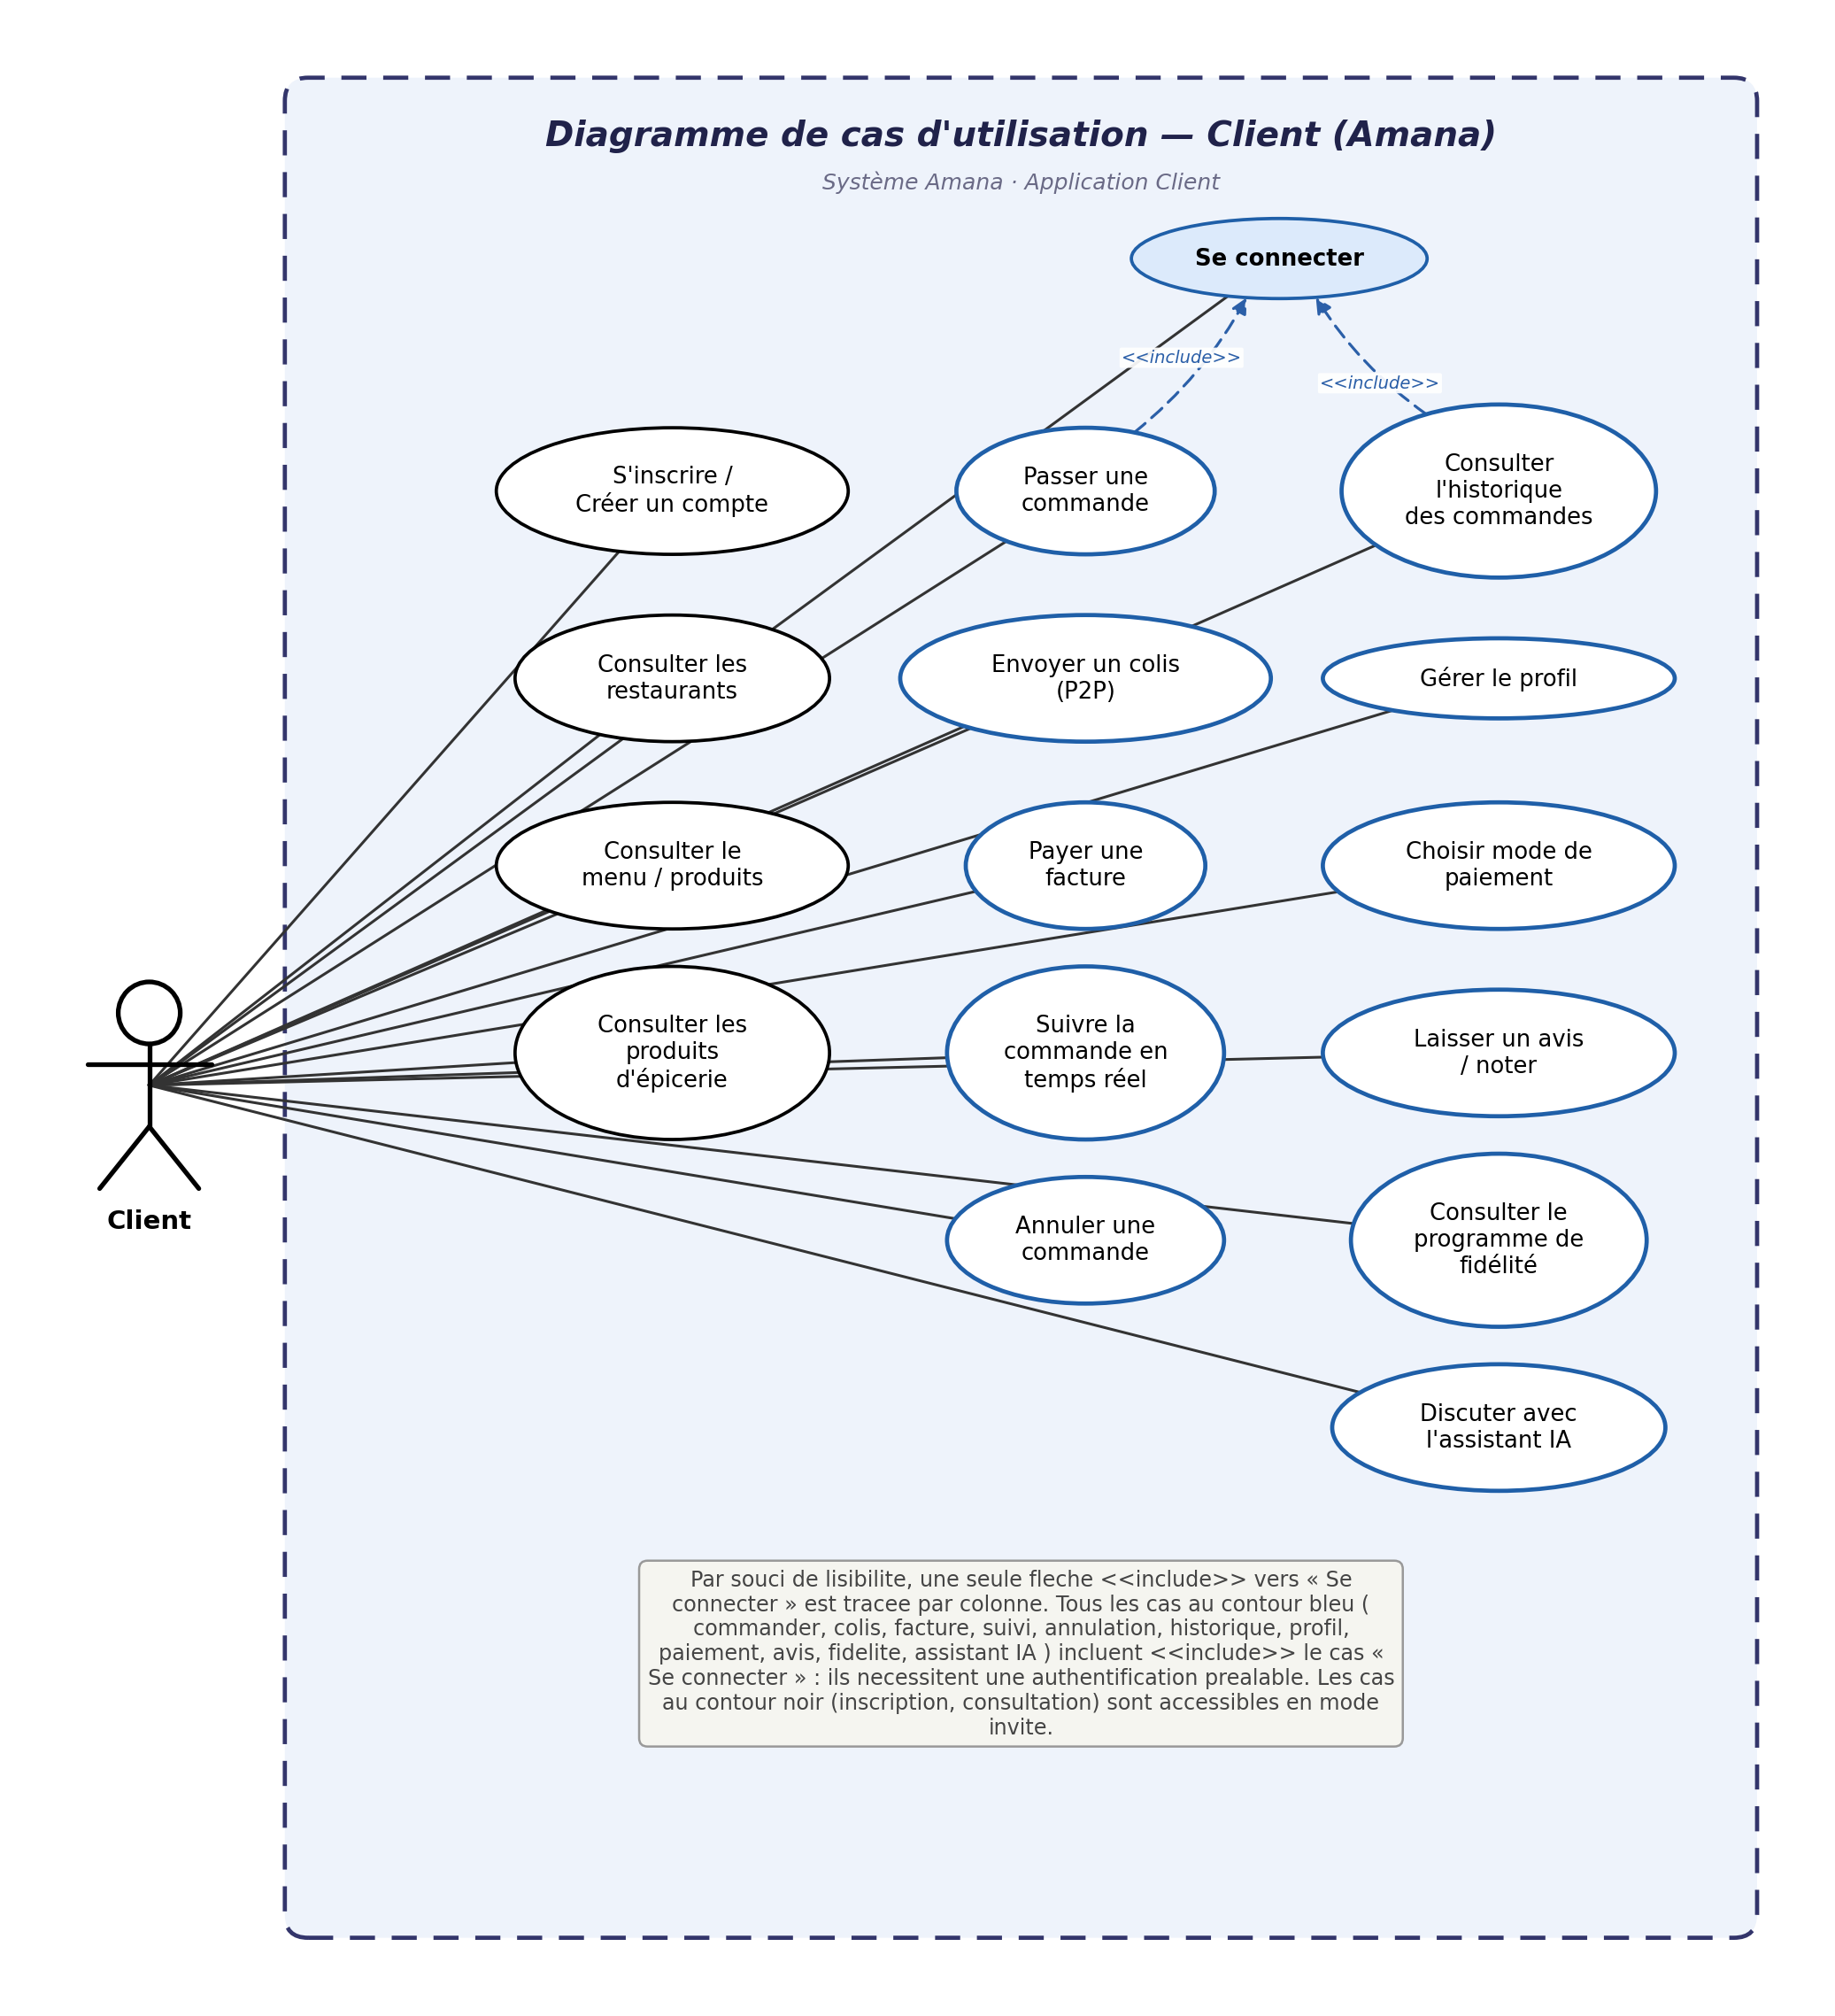
\includegraphics[width=\textwidth,height=0.9\textheight,keepaspectratio]{cas_utilisation_client_v2.png}}
    \caption{Diagramme de cas d'utilisation partie 1 : Client}
\end{figure}
\newpage

\begin{figure}[H]
    \centering
    \fbox{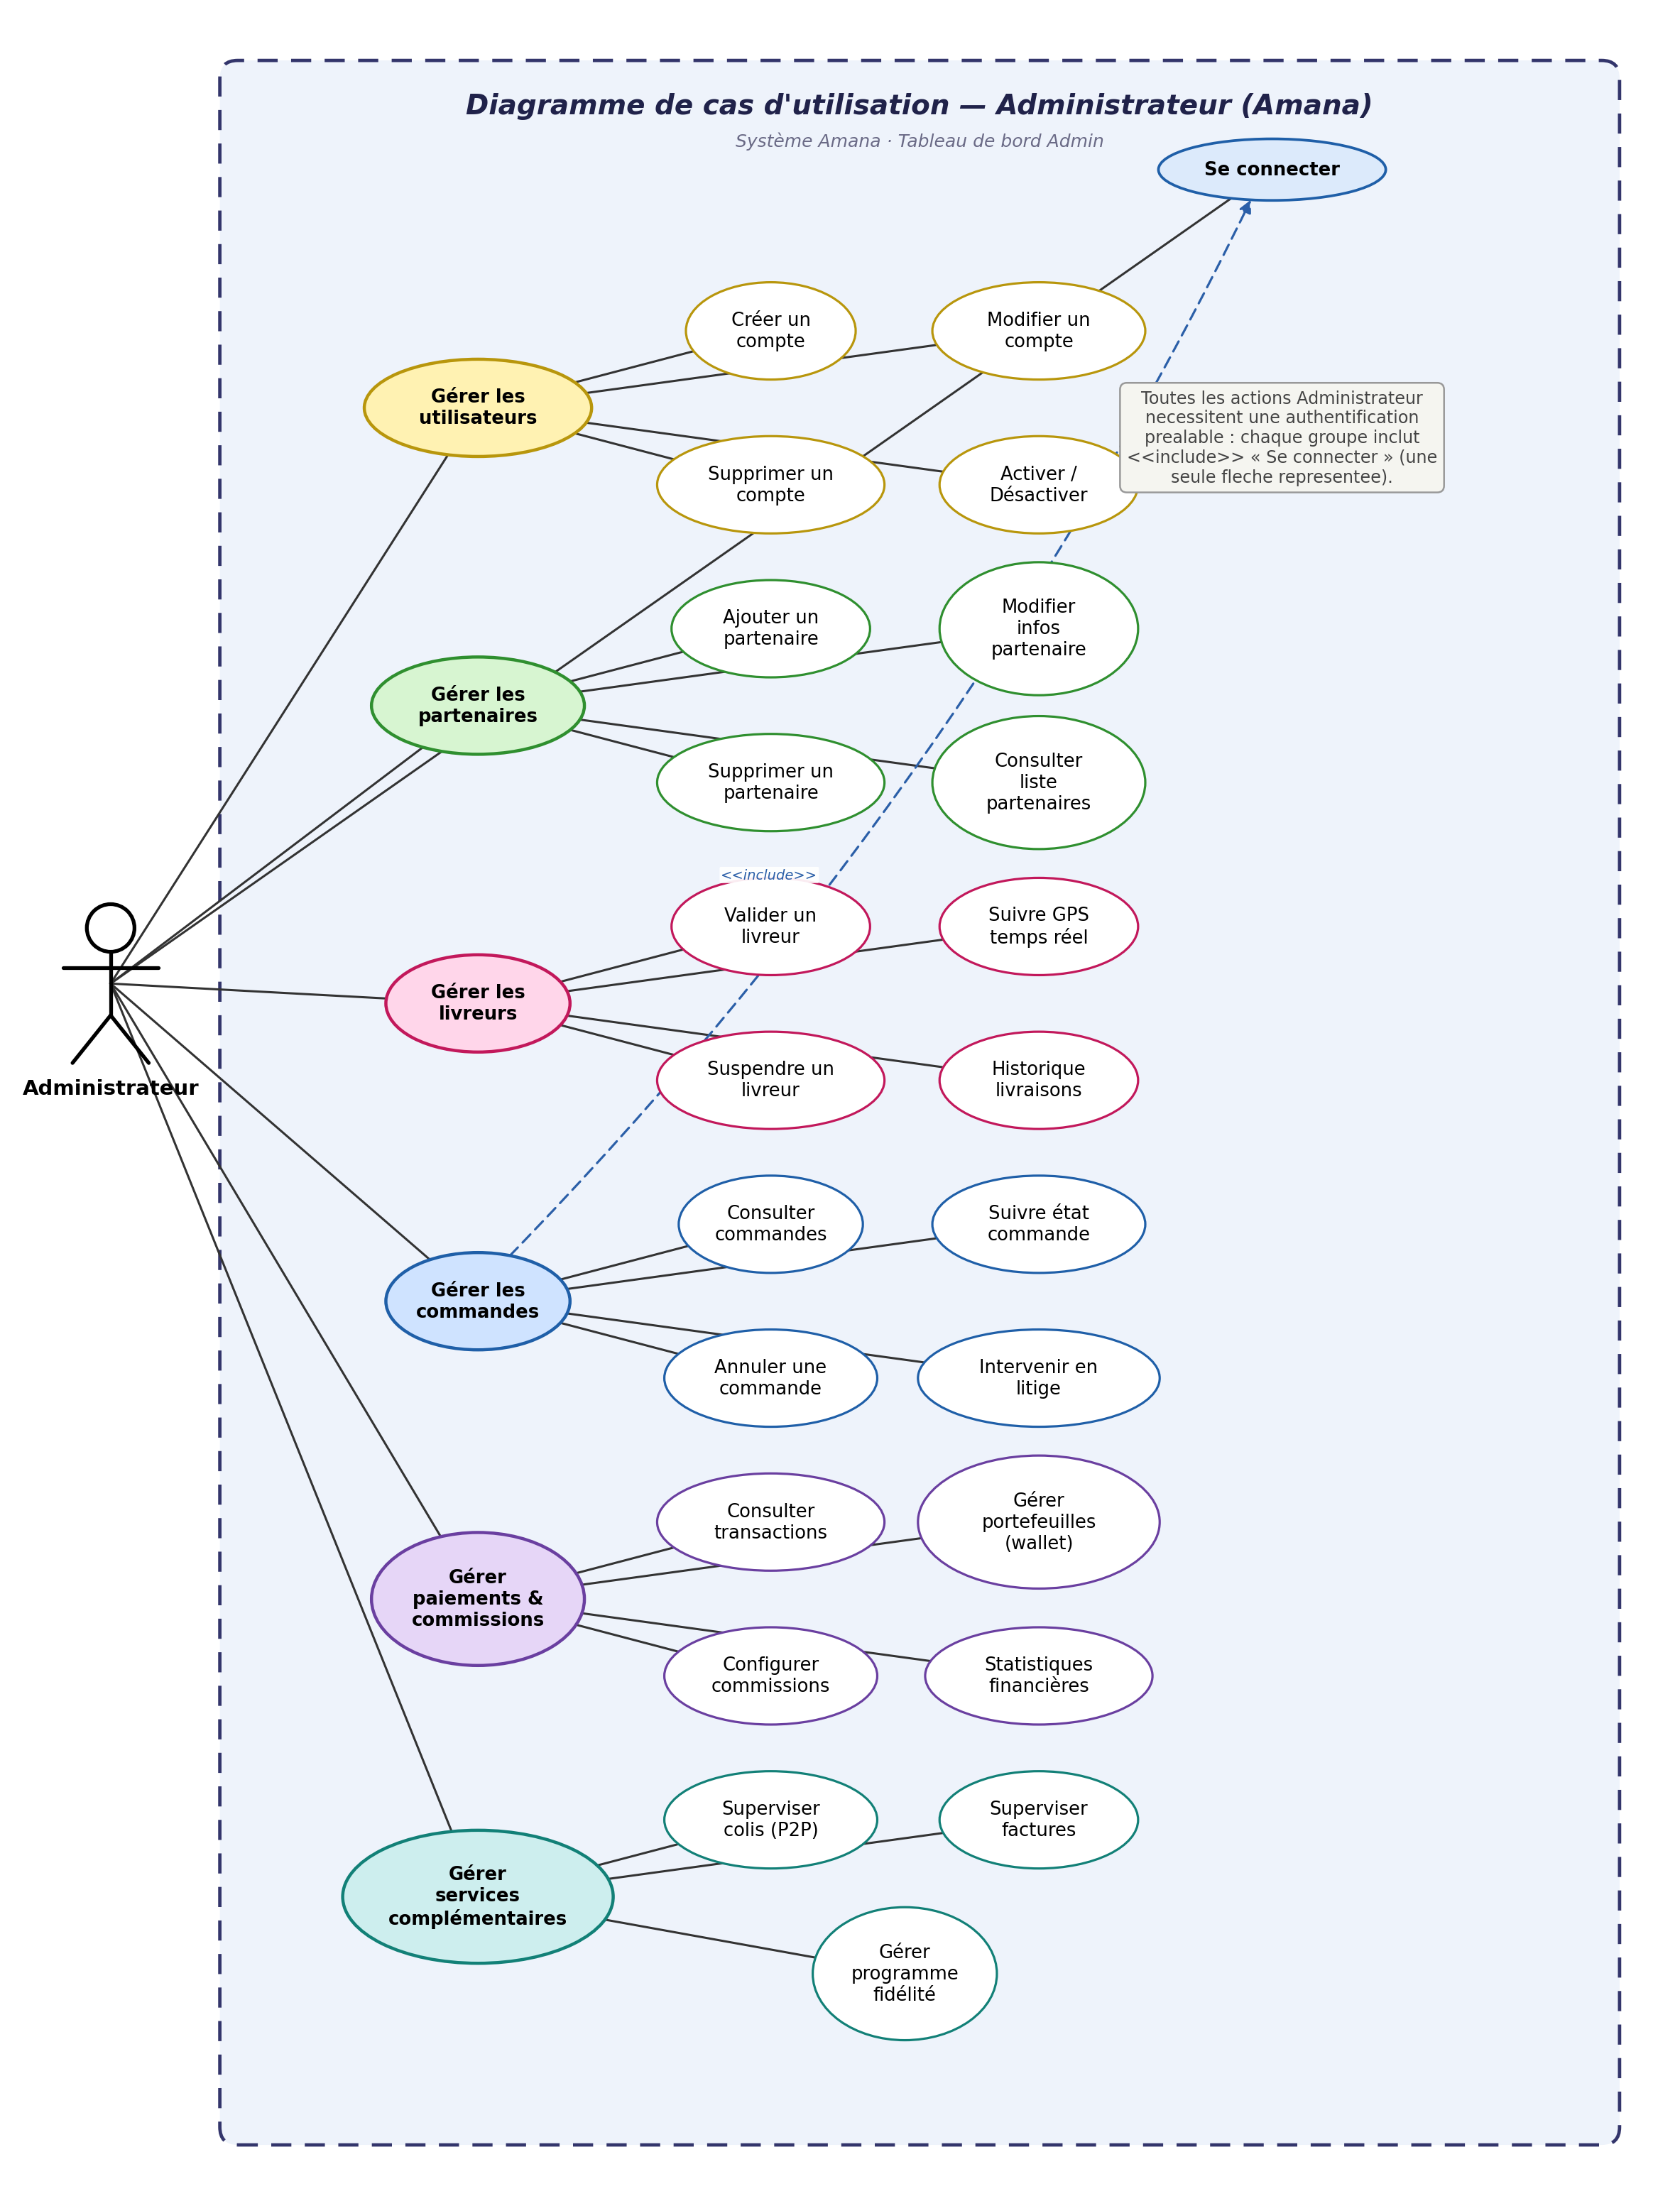
\includegraphics[width=\textwidth,height=0.9\textheight,keepaspectratio]{cas_utilisation_admin_v2.png}}
    \caption{Diagramme de cas d'utilisation partie 2 : Administrateur}
\end{figure}
\newpage

\begin{figure}[H]
    \centering
    \fbox{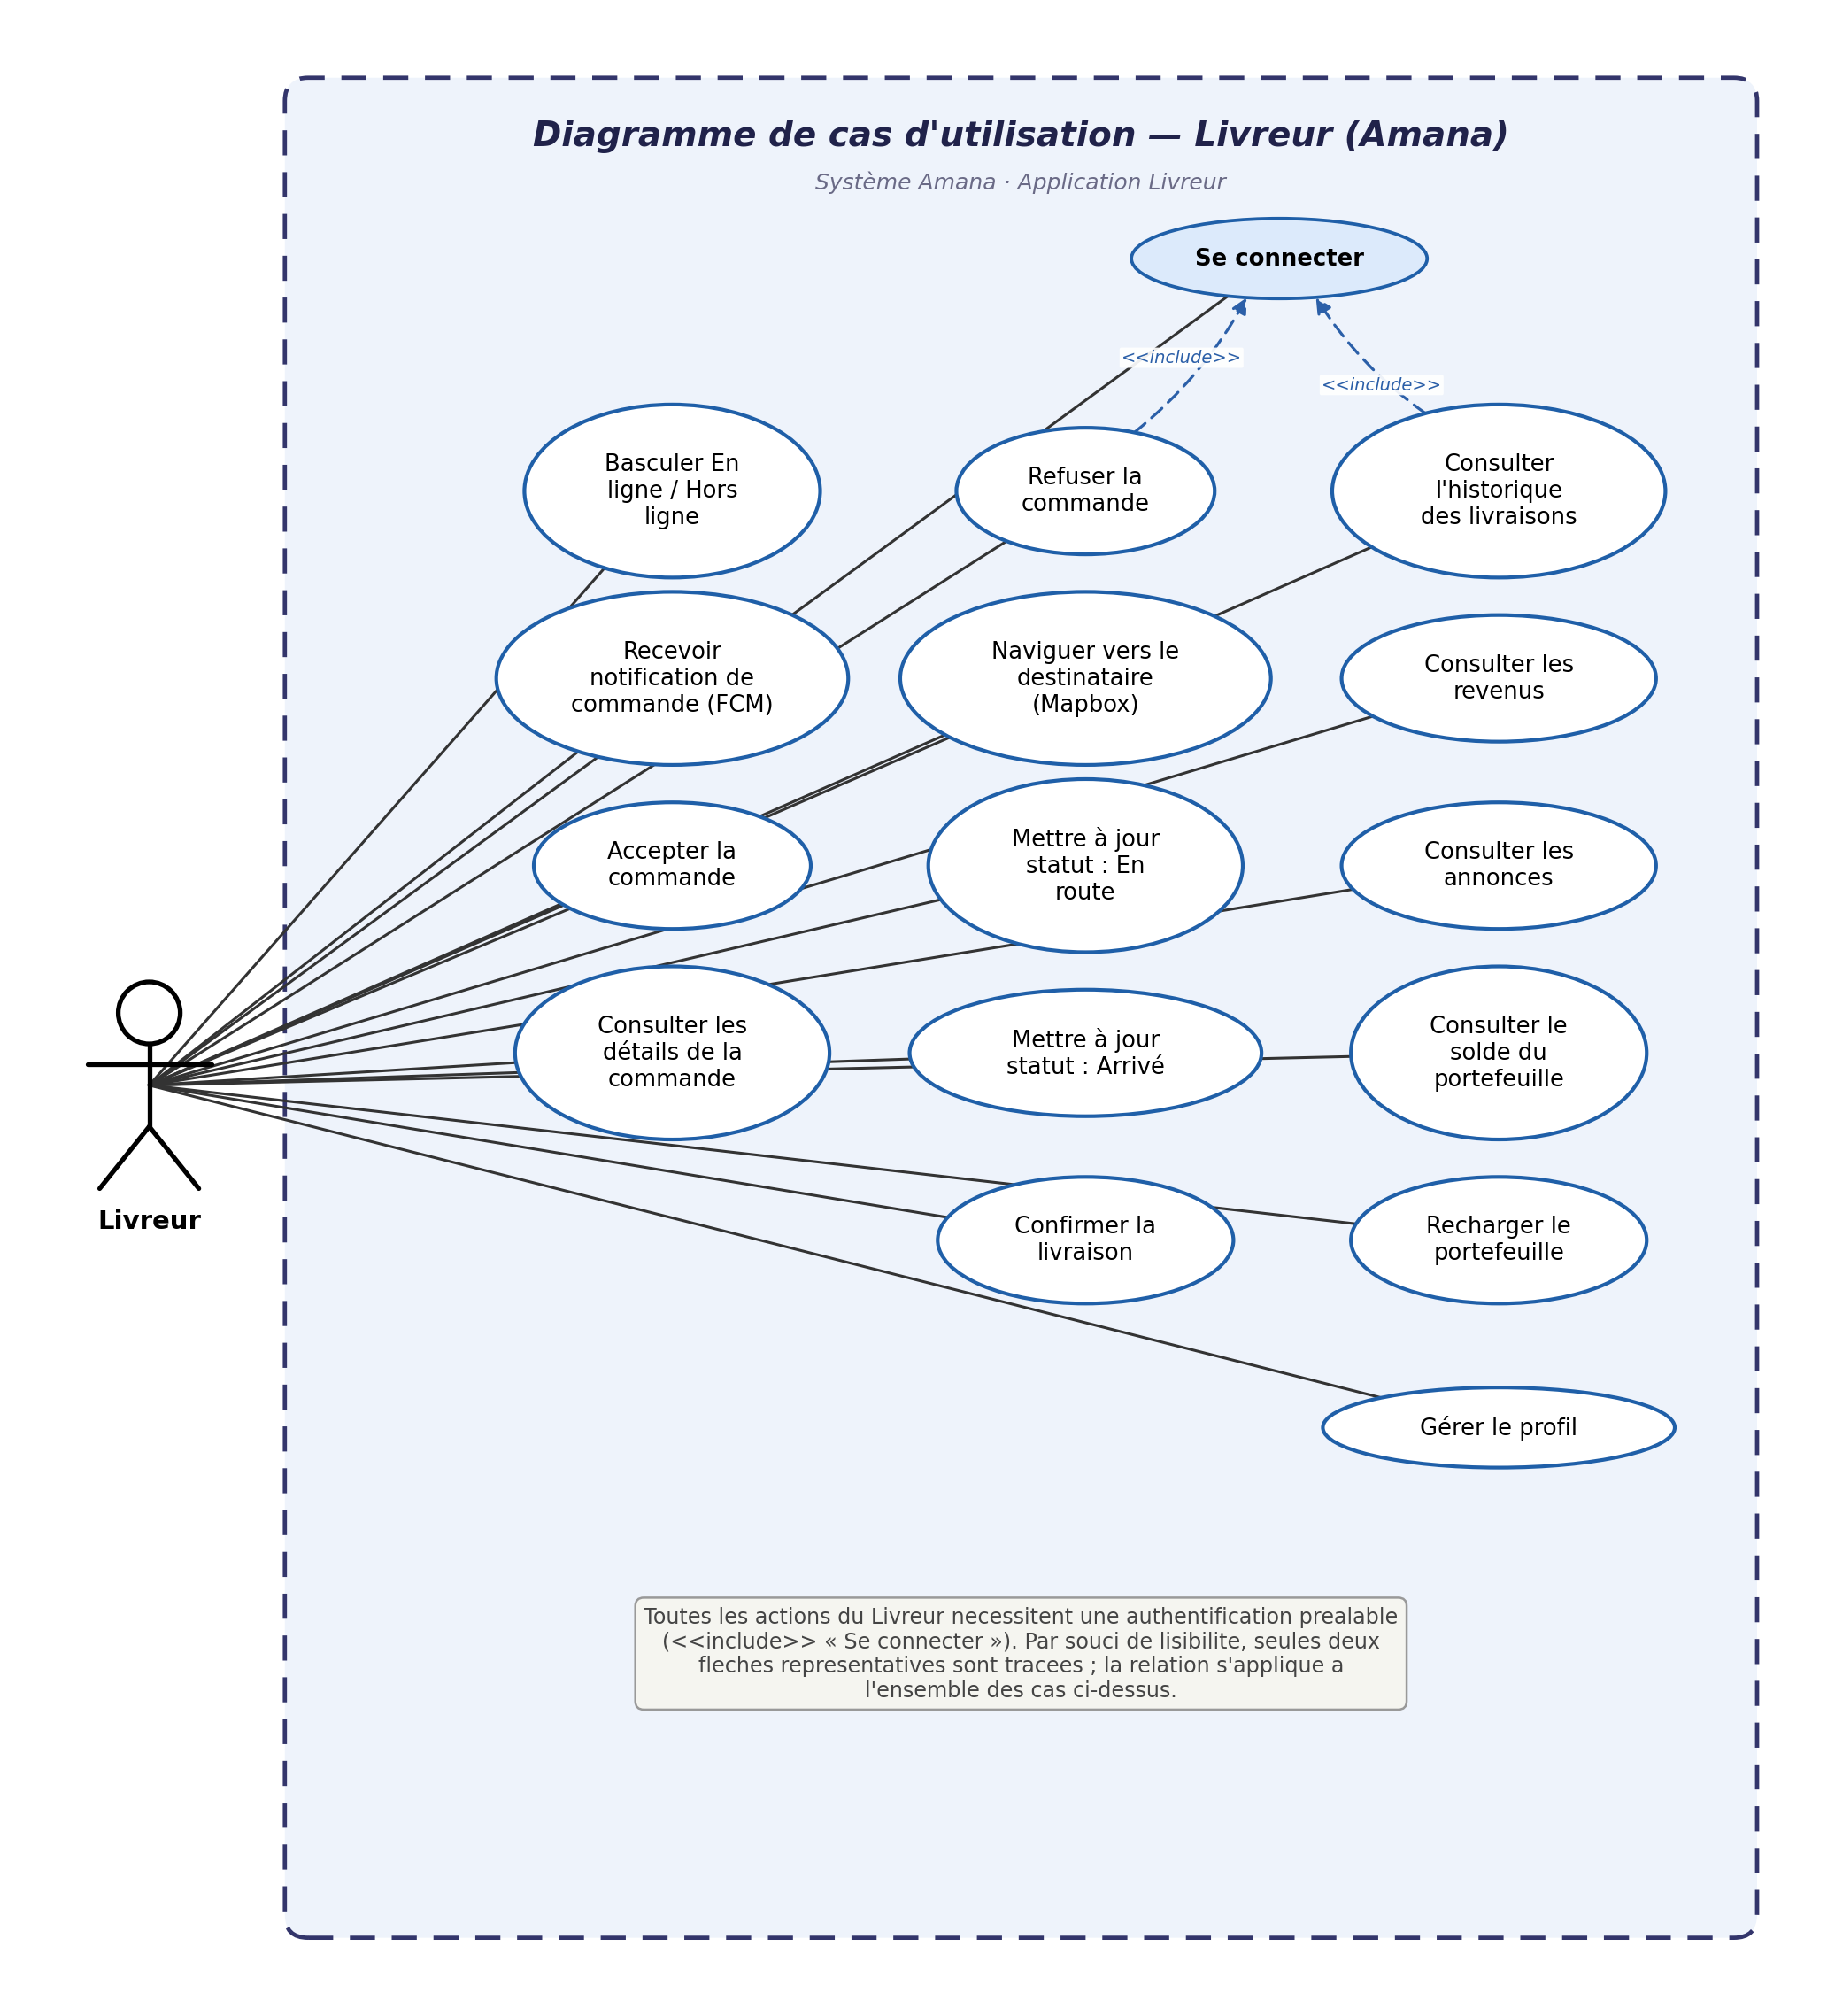
\includegraphics[width=\textwidth,height=0.9\textheight,keepaspectratio]{cas_utilisation_livreur_v2.png}}
    \caption{Diagramme de cas d'utilisation partie 3 : Livreur}
\end{figure}
\newpage

\begin{figure}[H]
    \centering
    \fbox{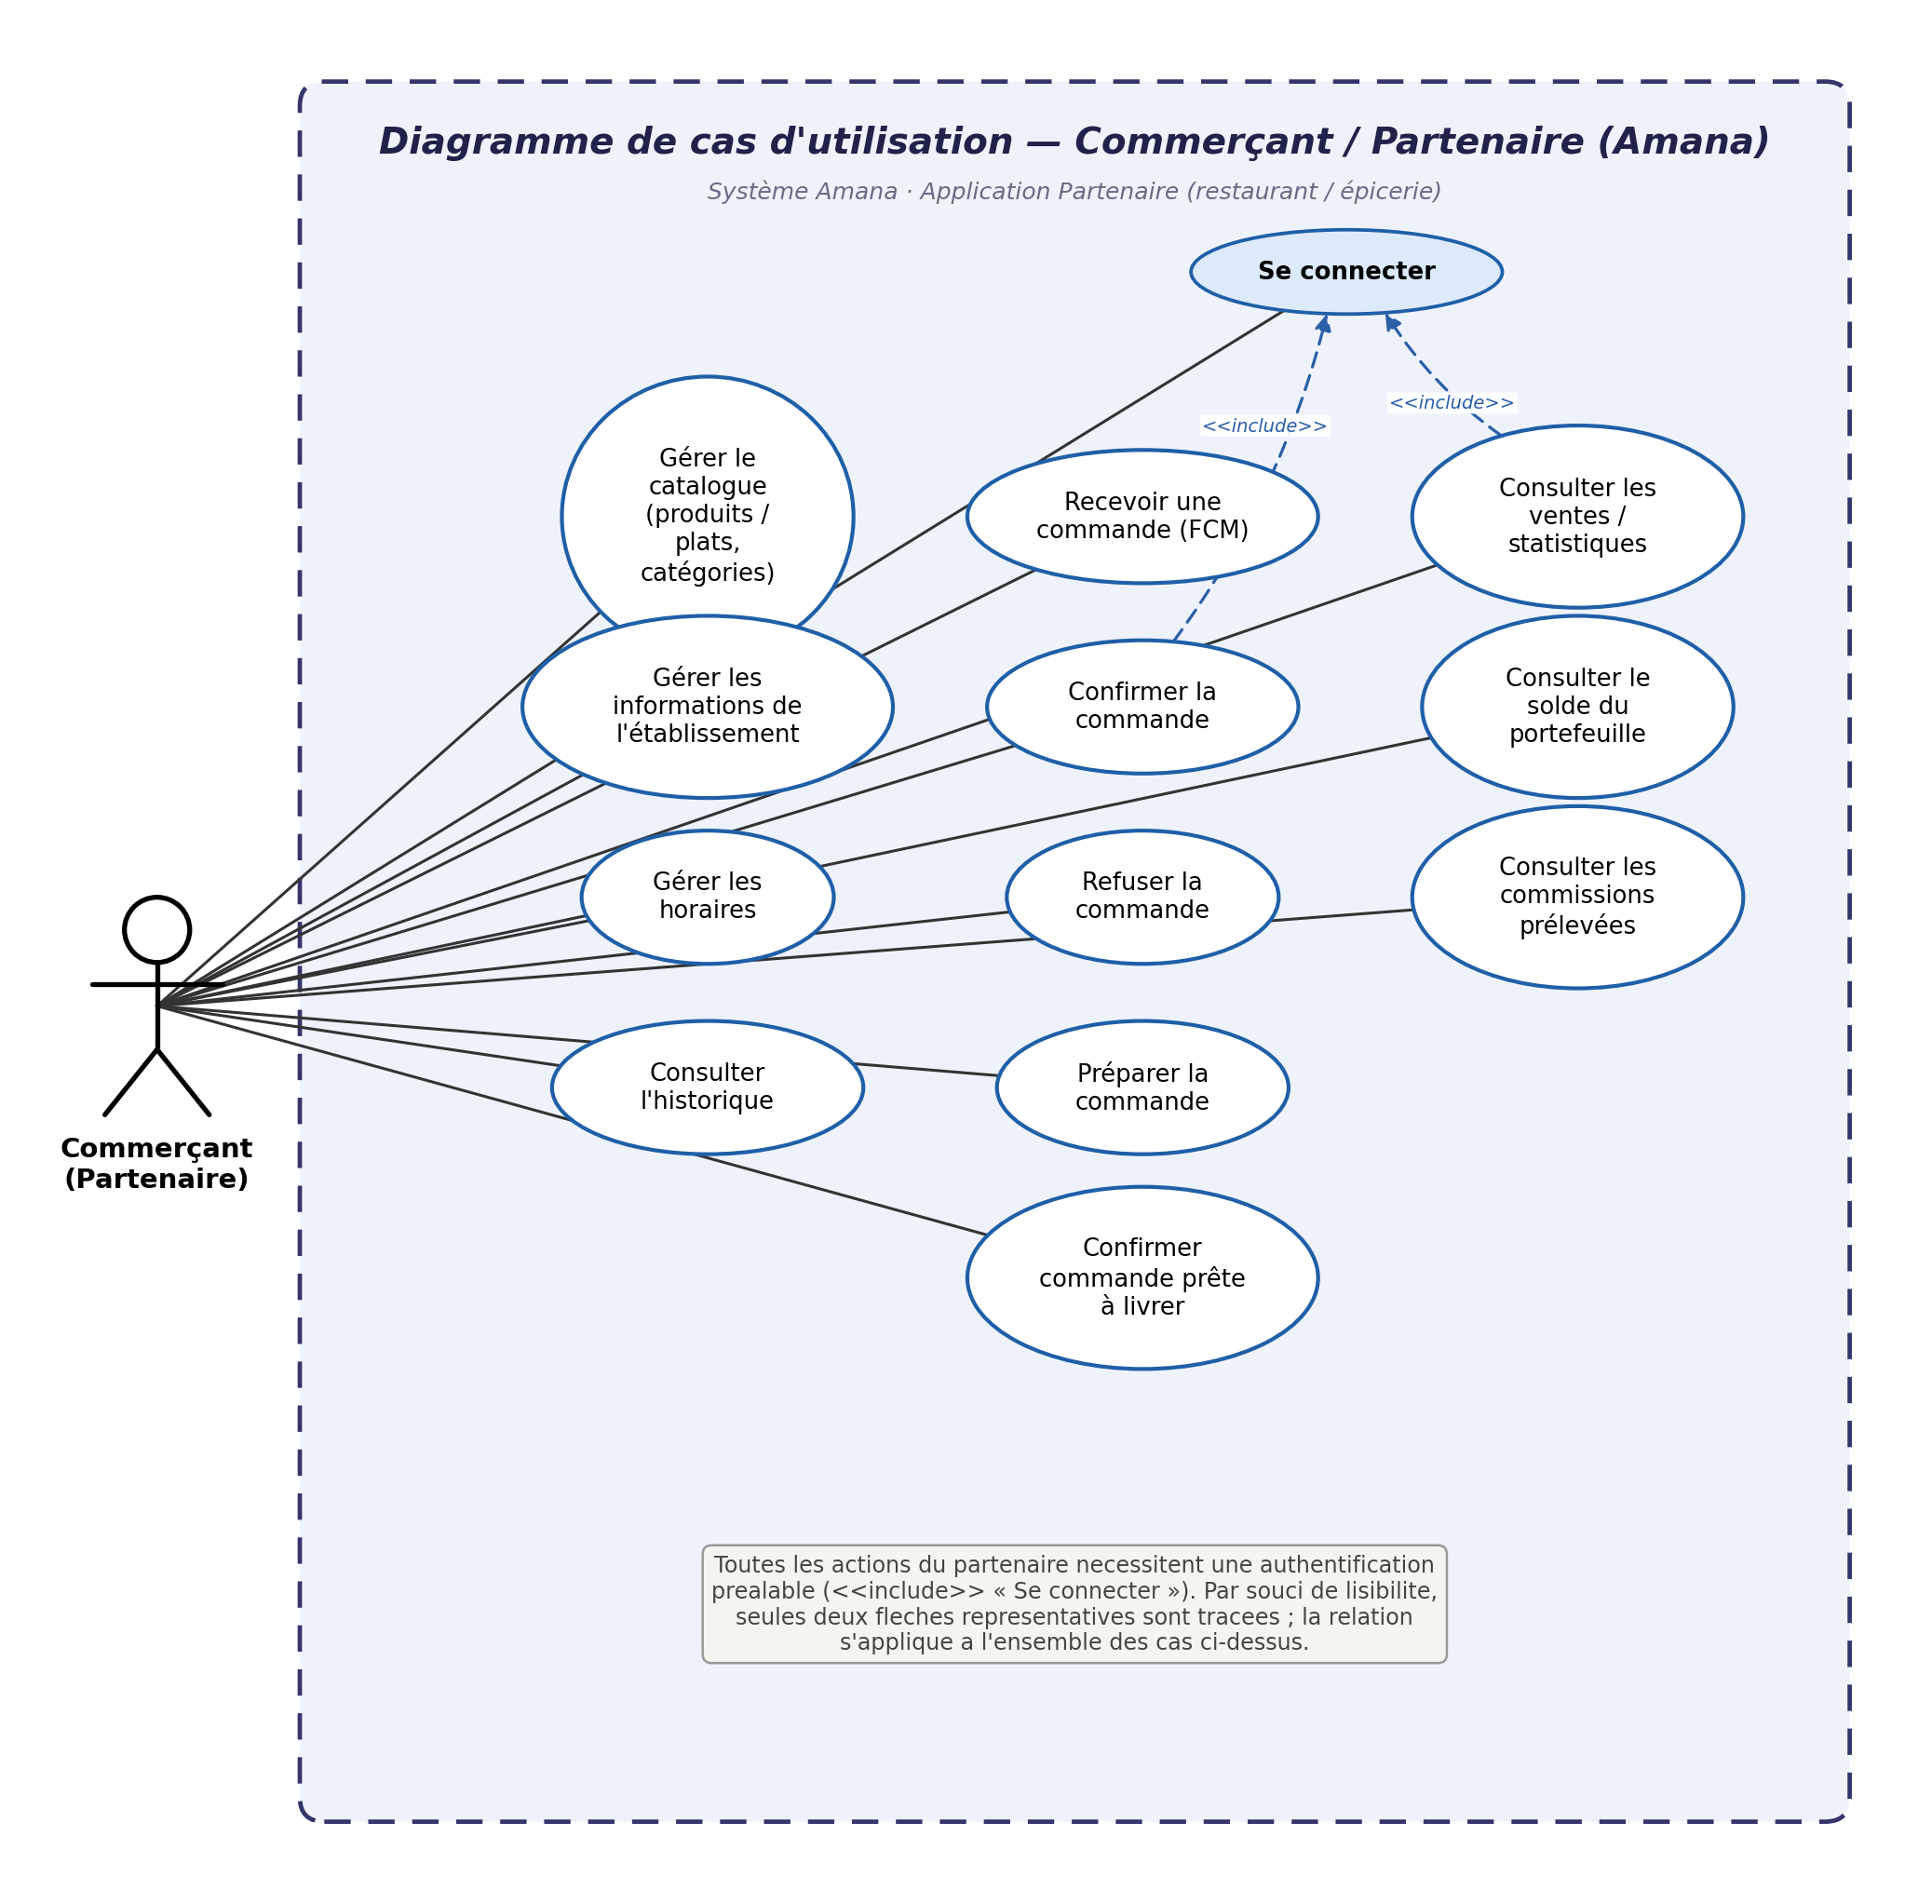
\includegraphics[width=\textwidth,height=0.9\textheight,keepaspectratio]{cas_utilisation_partenaire_v2.png}}
    \caption{Diagramme de cas d'utilisation partie 4 : Commerçant / Partenaire}
\end{figure}
\newpage

L'analyse de ces interactions montre une séparation claire des responsabilités. Le Client est le moteur de l'activité, déclenchant des processus de commande ou de livraison P2P. Le Commerçant et le Livreur agissent comme des exécutants opérationnels, tandis que l'Administrateur conserve une vue transversale pour garantir la fiabilité des échanges.

\subsubsection{Raffinement suivre la commande}
Pour garantir une expérience utilisateur fluide, nous avons procédé à un raffinement des cas d'utilisation les plus complexes.

\begin{figure}[H]
    \centering
    \fbox{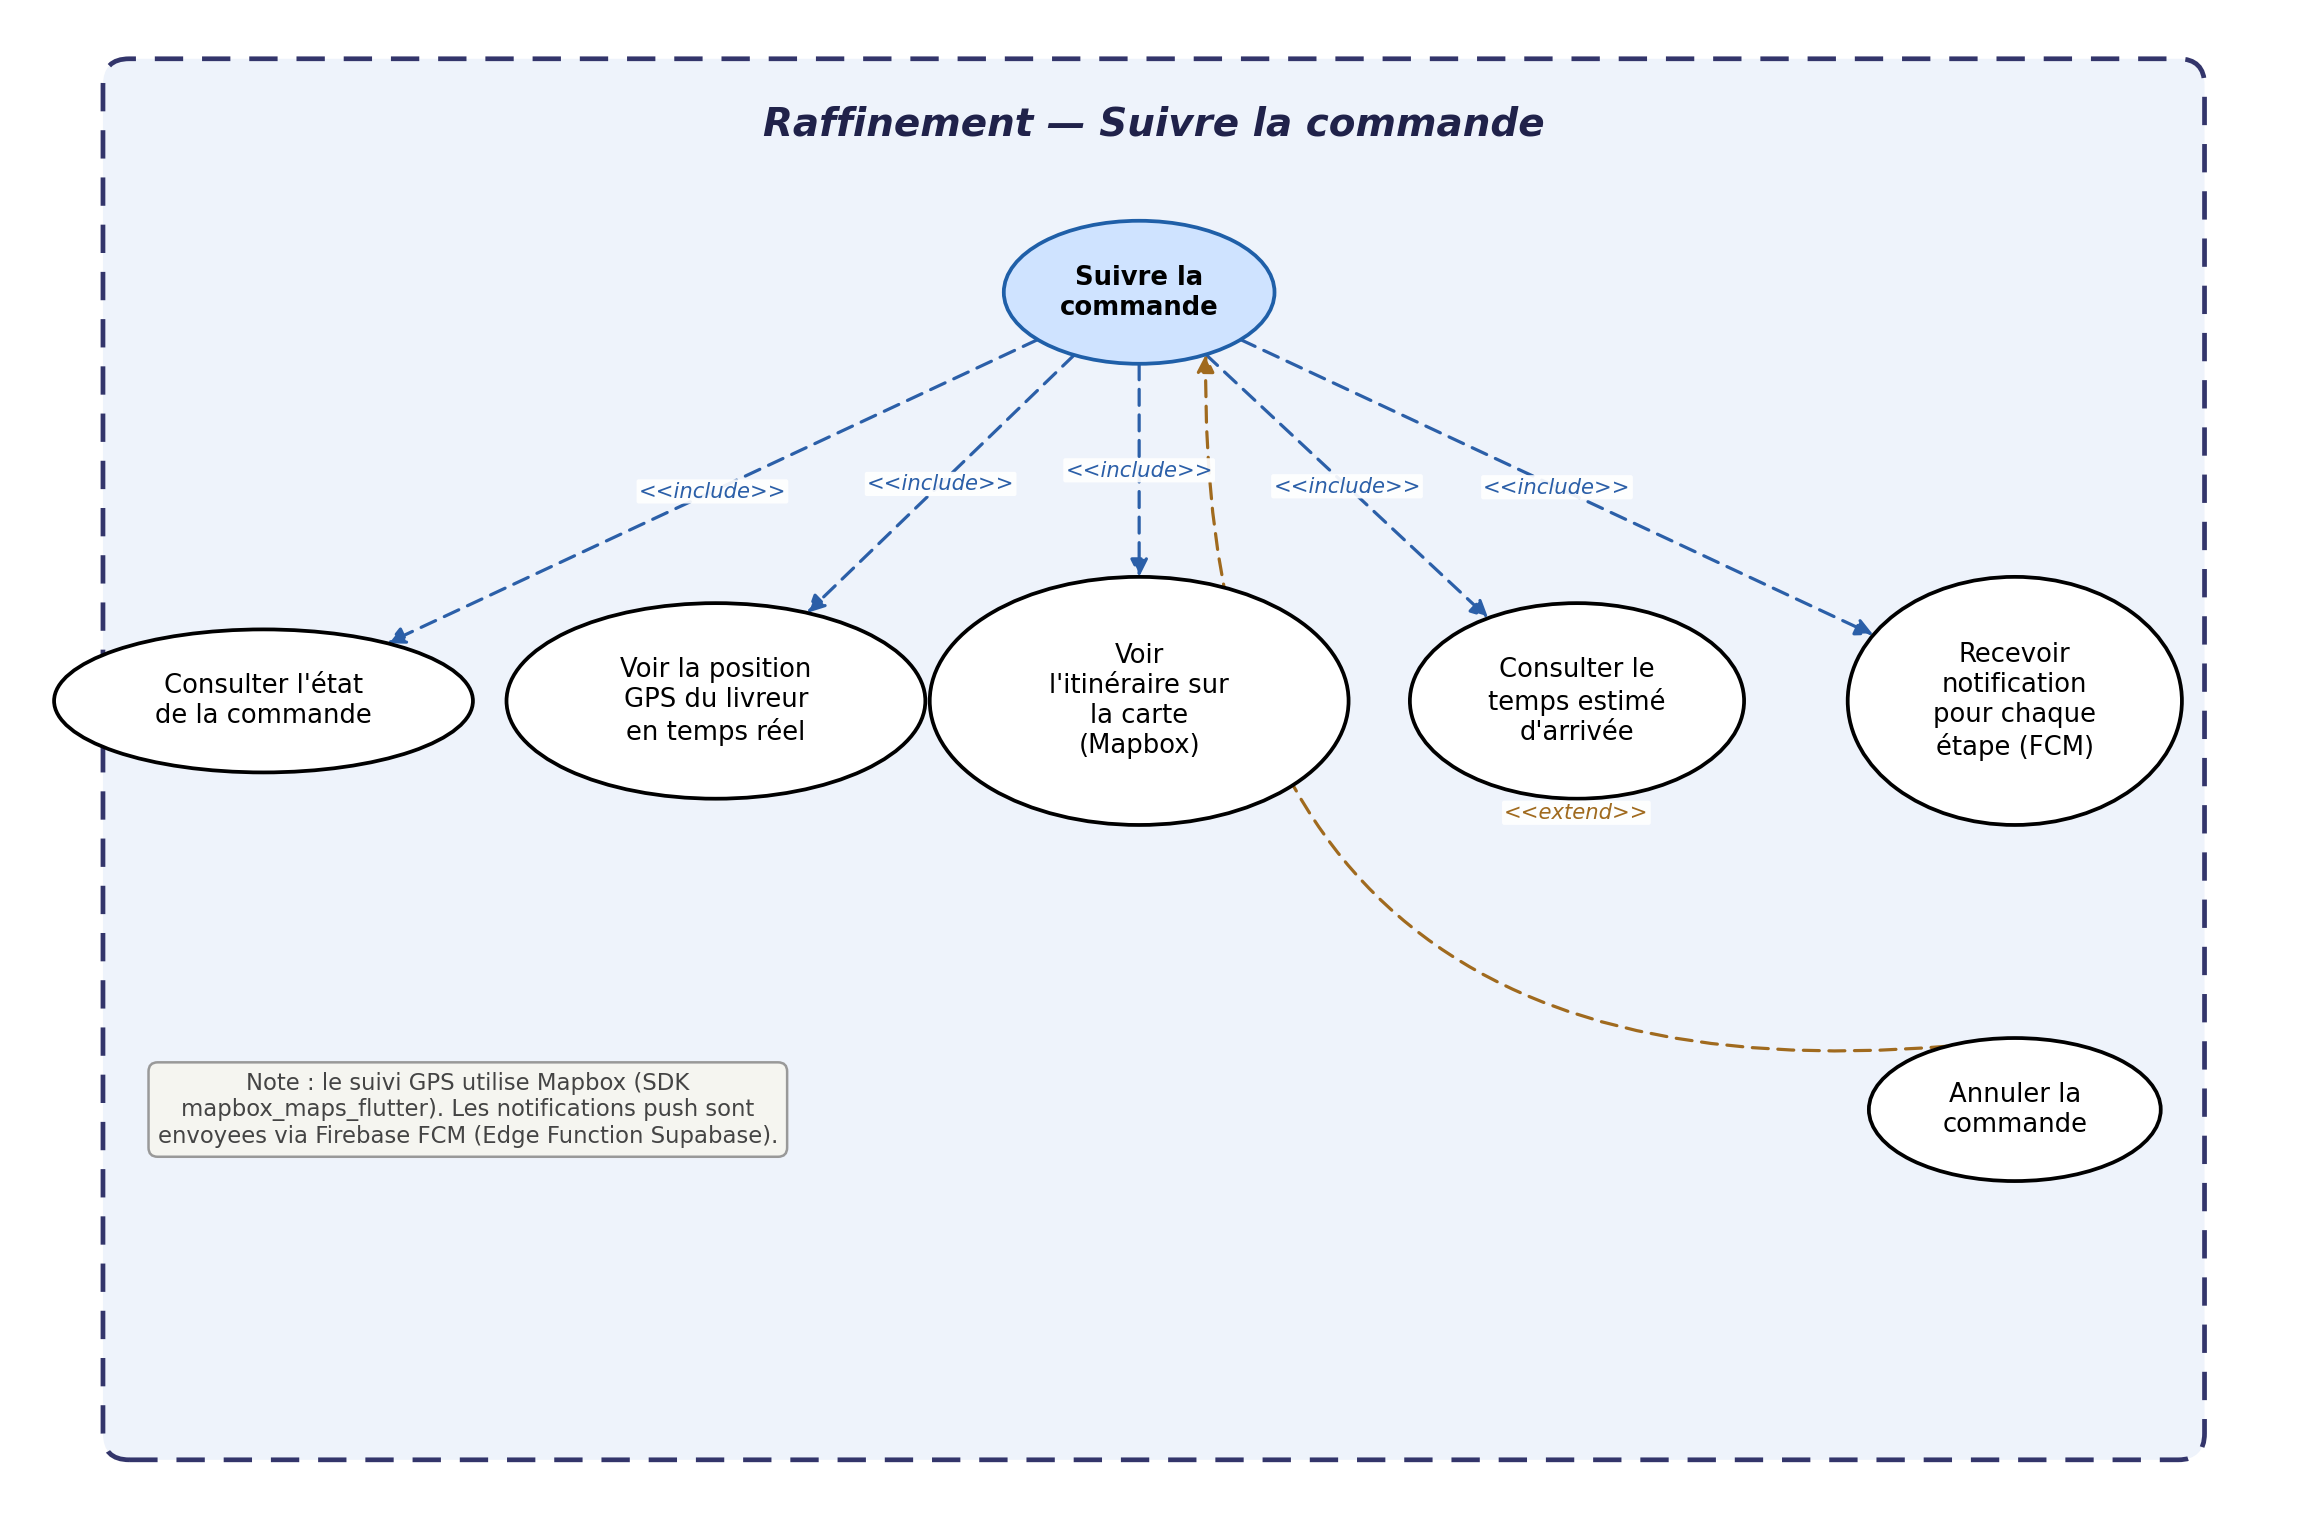
\includegraphics[width=\textwidth,height=0.6\textheight,keepaspectratio]{raffinement_suivre_commande_v2.png}}
    \caption{Raffinement : suivre la commande}
\end{figure}
\begin{table}[H]
\centering
\renewcommand{\arraystretch}{1.4}
\begin{tabular}{|l|l|p{7cm}|}
\hline
\textbf{Cas d'utilisation} & \textbf{Type} & \textbf{Description} \\
\hline
Suivre la commande & Cas principal &
Le client dispose d'un écran dédié pour
surveiller en direct l'avancement de sa
livraison, regroupant toutes les informations
utiles en un seul endroit. \\
\hline
Consulter l'état de la commande & Inclusion &
Un indicateur de progression affiche
l'étape en cours parmi les huit statuts
possibles du système, de la confirmation
jusqu'à la livraison finale. \\
\hline
Voir la position GPS du livreur & Inclusion &
La localisation du livreur est mise à jour
à chaque déplacement d'environ 30 mètres
et apparaît sous forme de marqueur mobile
sur la carte. \\
\hline
Voir l'itinéraire sur la carte & Inclusion &
Le trajet entre le livreur et le point
de livraison est dessiné automatiquement
sur la carte intégrée via le SDK Mapbox. \\
\hline
Consulter le temps estimé d'arrivée & Inclusion &
Sur la base de la position GPS actuelle
du livreur, le système calcule et affiche
une durée approximative avant l'arrivée. \\
\hline
Recevoir une notification à chaque étape & Inclusion &
À chaque changement de statut, une alerte
est envoyée automatiquement sur le téléphone
du client grâce à Firebase FCM, déclenché
par une fonction côté serveur Supabase. \\
\hline
Annuler la commande & Extension &
Tant que la commande n'a pas été prise
en charge, le client peut l'annuler en
indiquant obligatoirement la raison de
sa décision. \\
\hline
\end{tabular}
\caption{Description textuelle du raffinement : Suivre la commande}
\end{table}

\subsubsection{Raffinement: passer une commande}

\begin{figure}[H]
    \centering
    \fbox{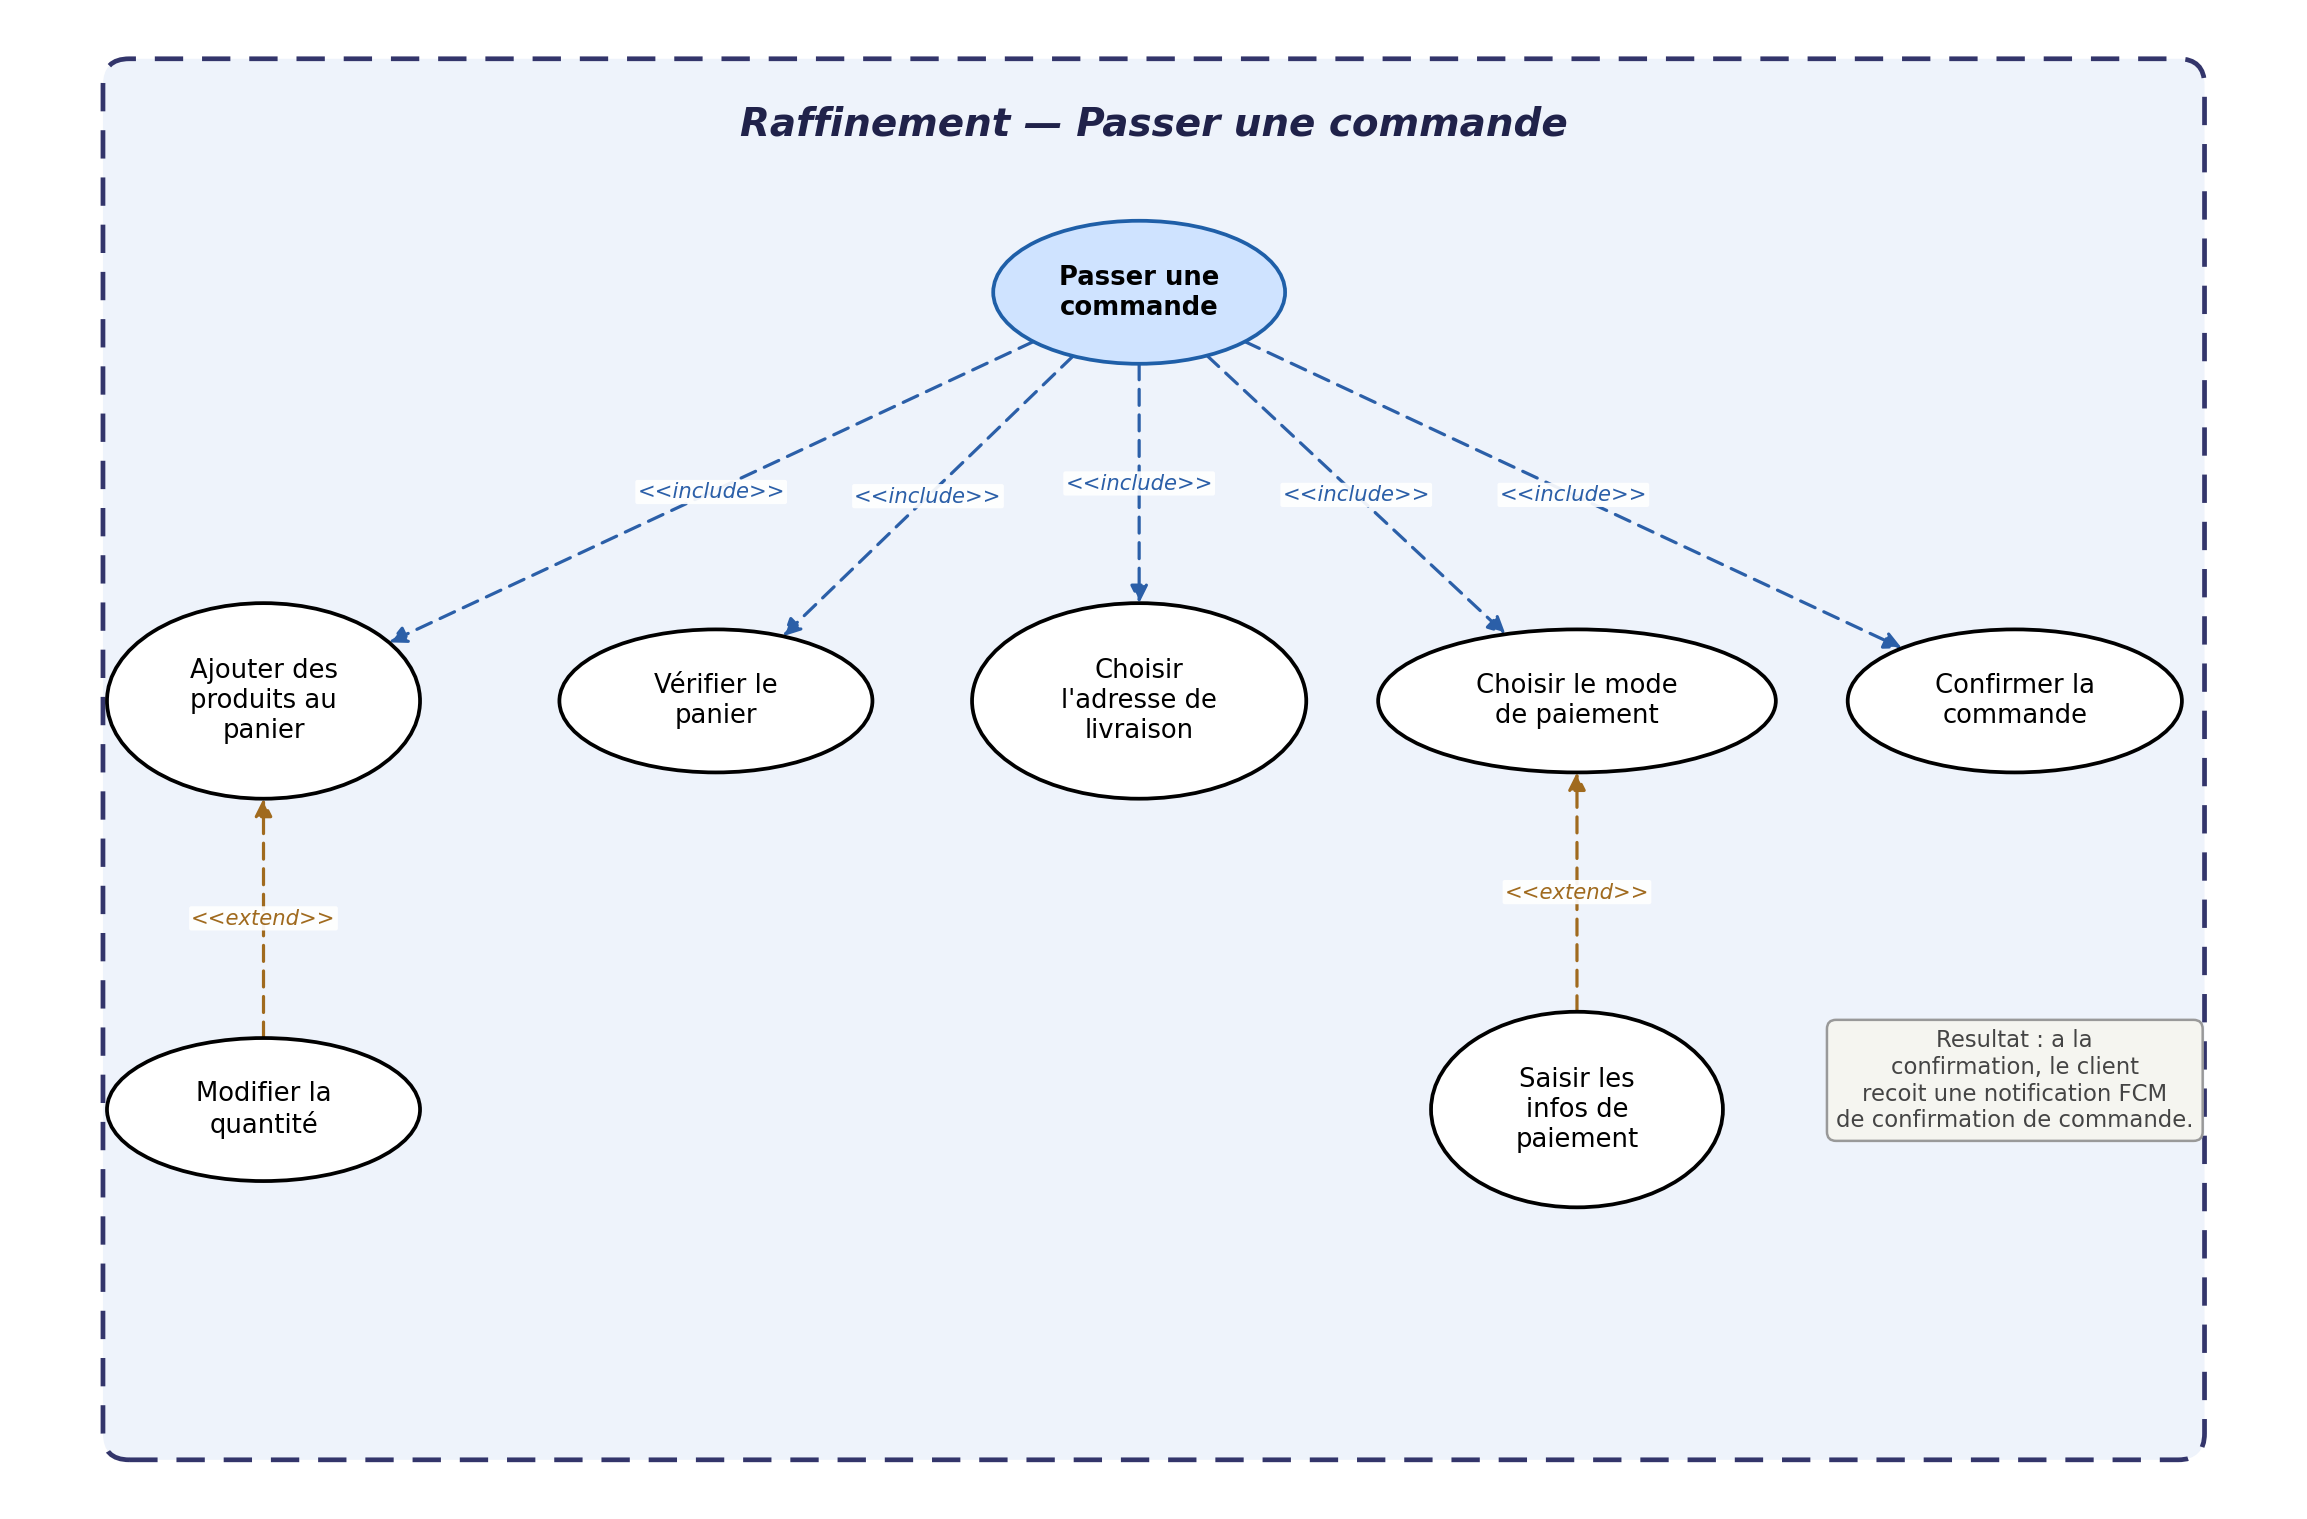
\includegraphics[width=\textwidth,height=0.6\textheight,keepaspectratio]{raffinement_passer_commande_v2.png}}
    \caption{Raffinement : Passer commande}
\end{figure}
\begin{table}[H]
\centering
\renewcommand{\arraystretch}{1.4}
\begin{tabular}{|l|l|p{7cm}|}
\hline
\textbf{Cas d'utilisation} & \textbf{Type} & \textbf{Description} \\
\hline
Passer une commande & Cas principal &
Le client réalise l'ensemble des étapes
nécessaires pour soumettre sa commande,
depuis la sélection des articles jusqu'à
la validation finale. \\
\hline
Ajouter des produits au panier & Inclusion &
Le client sélectionne les articles souhaités
depuis le menu du restaurant ou du commerce,
avec la possibilité de personnaliser chaque
plat selon les options disponibles. \\
\hline
Modifier la quantité & Extension &
Depuis le panier, le client peut augmenter
ou réduire le nombre d'unités de chaque
article avant de passer à l'étape suivante. \\
\hline
Vérifier le panier & Inclusion &
Avant de confirmer, le client consulte
le récapitulatif de sa commande avec le
détail des articles, leurs options choisies
et le montant total à régler. \\
\hline
Choisir l'adresse de livraison & Inclusion &
Le client saisit ou sélectionne l'adresse
à laquelle il souhaite recevoir sa commande,
à partir de ses adresses enregistrées
ou via la carte. \\
\hline
Choisir le mode de paiement & Inclusion &
Le client indique comment il souhaite régler
sa commande, selon les moyens disponibles
proposés par la plateforme. \\
\hline
Saisir les infos de paiement & Extension &
Si le mode de paiement choisi le nécessite,
le client complète les informations requises
pour finaliser la transaction. \\
\hline
Confirmer la commande & Inclusion &
Le client valide définitivement sa commande.
À ce moment, une notification de confirmation
lui est envoyée automatiquement via
Firebase FCM. \\
\hline
\end{tabular}
\caption{Description textuelle du raffinement : Passer une commande}
\end{table}
\clearpage
\subsection{Ajouter un plat:}
\begin{figure}[H]
    \centering
    \fbox{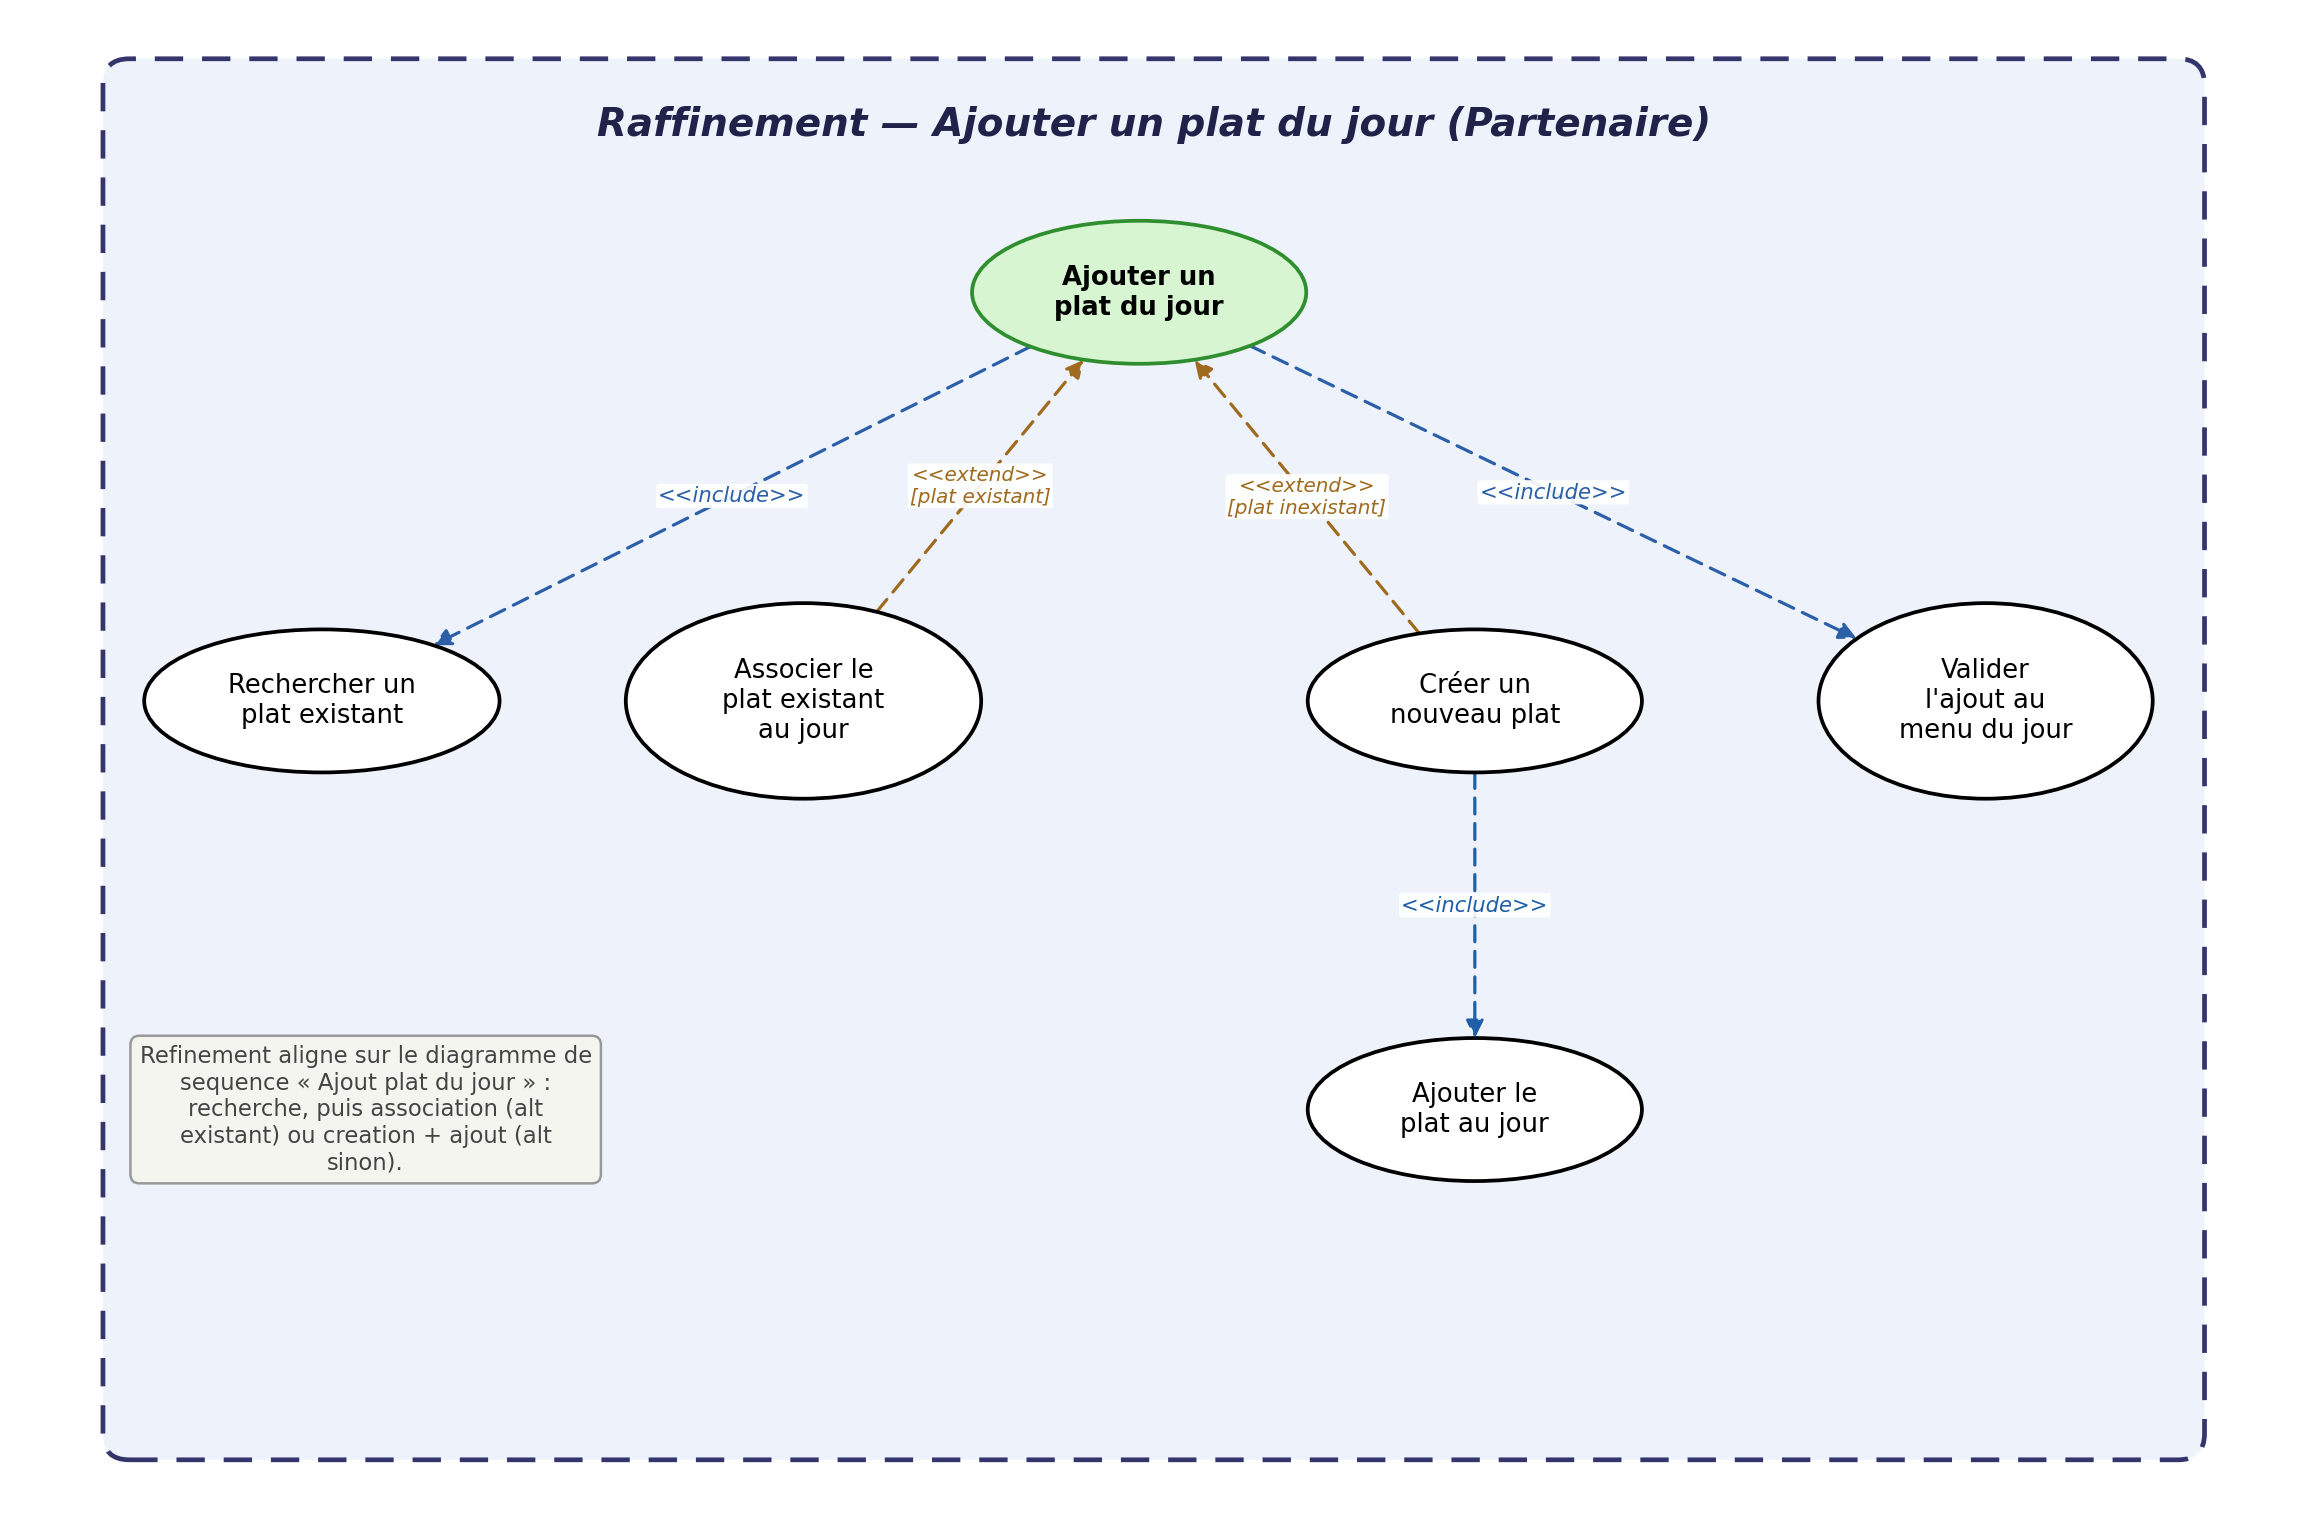
\includegraphics[width=\textwidth,height=0.75\textheight,keepaspectratio]{raffinement_ajout_plat_jour.png}}
    \caption{Raffinement : Ajouter un plat du jour}
\end{figure}

\subsection{Livrer une commande:}
\begin{figure}[H]
    \centering
    \fbox{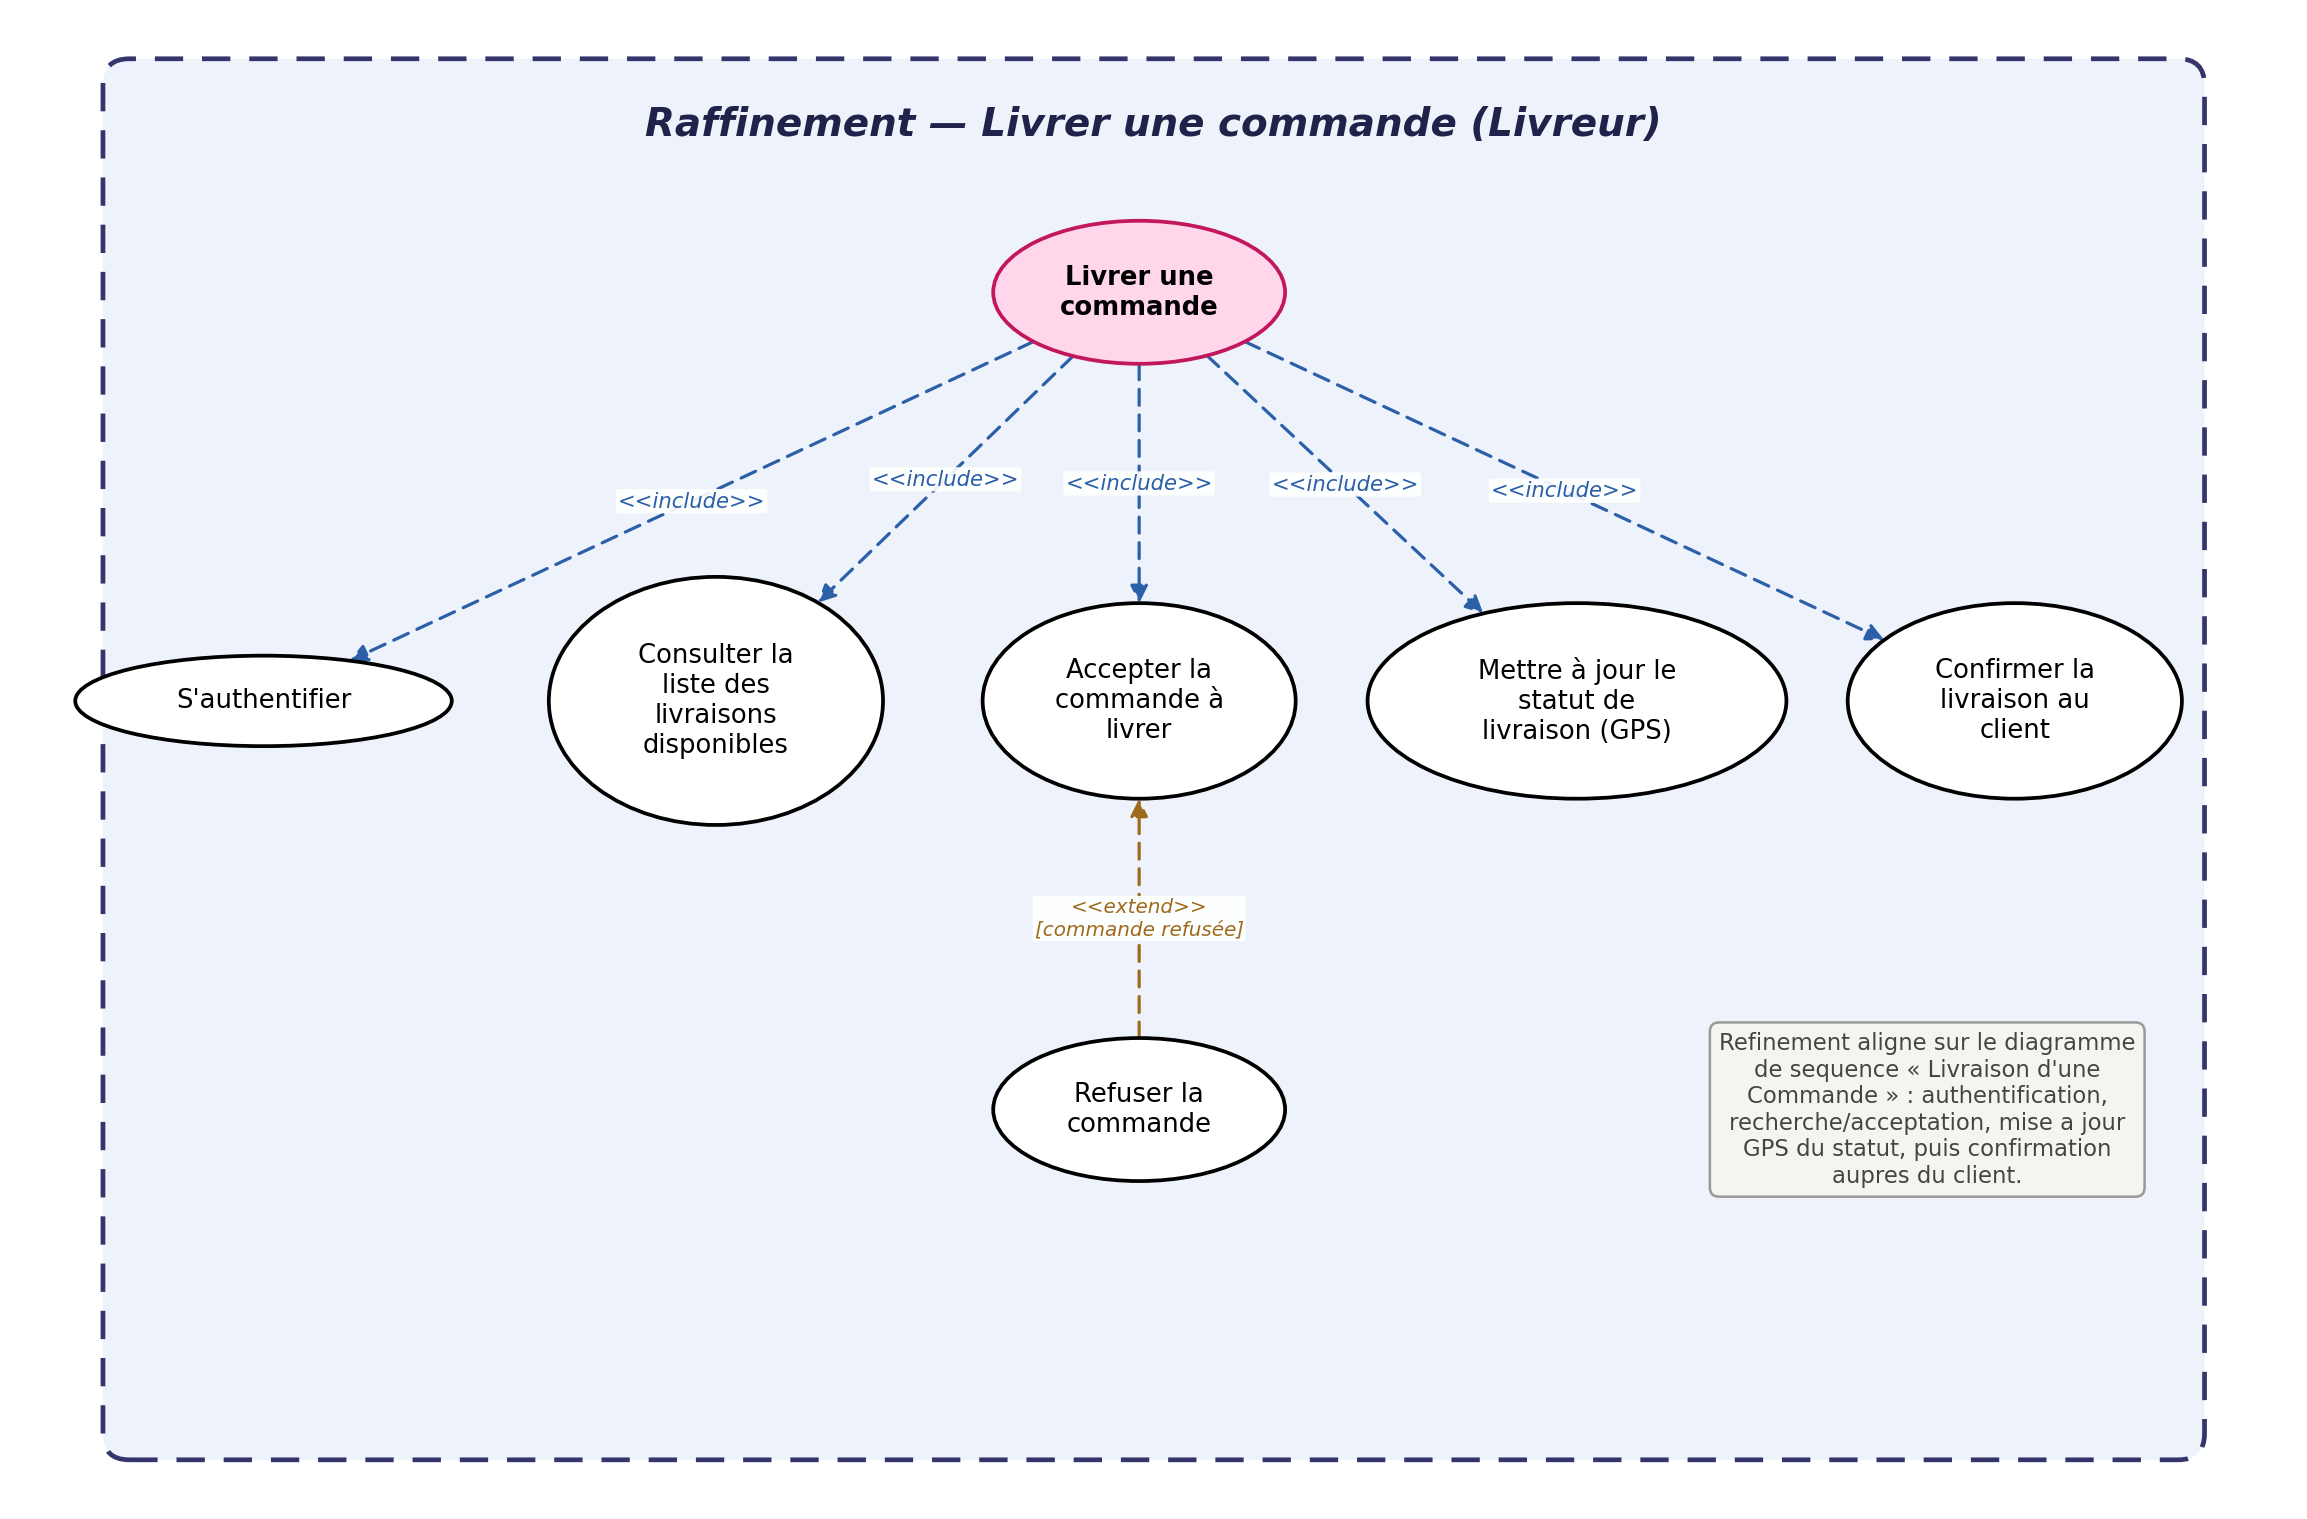
\includegraphics[width=\textwidth,height=0.75\textheight,keepaspectratio]{raffinement_livraison_commande.png}}
    \caption{Raffinement : Livrer une commande}
\end{figure}


\section{Diagramme de classe :}
Le diagramme de classe présente la structure statique de notre système et l'organisation logique de la base de données PostgreSQL gérée sous Supabase.

\begin{figure}[H]
    \centering
    \fbox{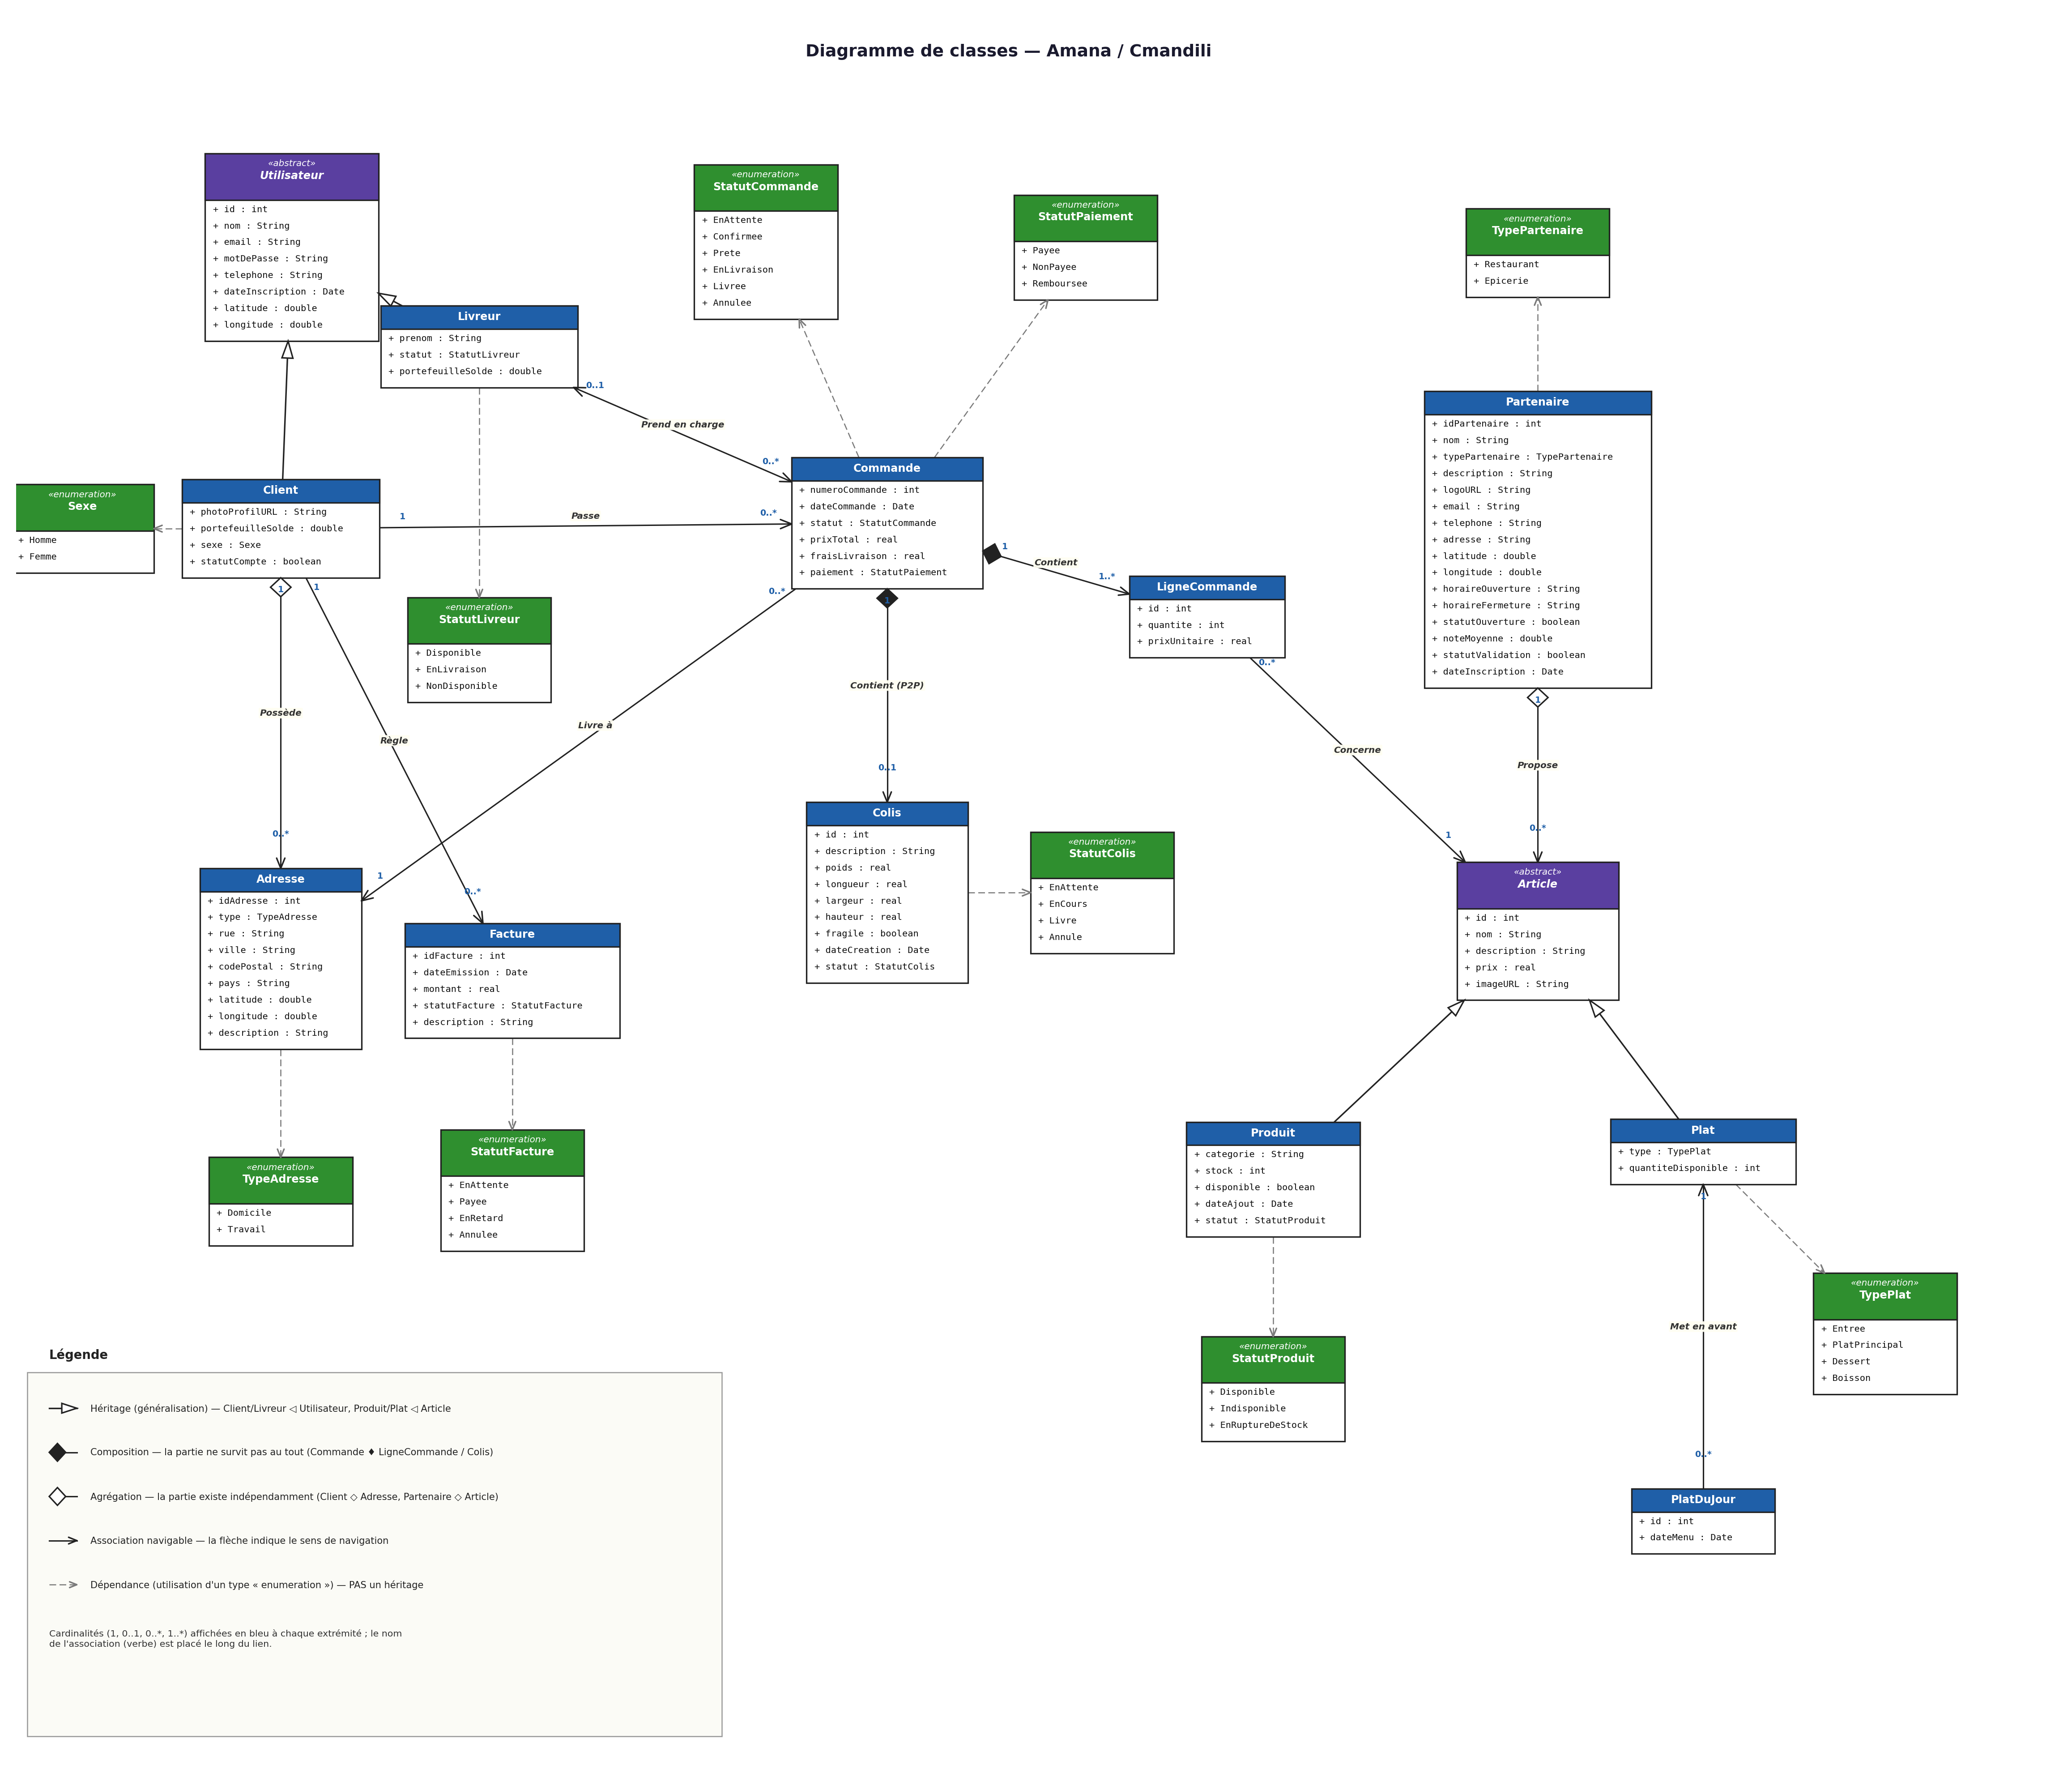
\includegraphics[width=\textwidth,height=0.85\textheight,keepaspectratio]{diagramme_classe_v2_full.png}}
    \caption{Diagramme de classe}
\end{figure}
\newpage

Le diagramme de classe constitue la colonne vertébrale technique de notre application. Il représente la structure statique du système et définit comment les données sont organisées au sein de notre base PostgreSQL sur Supabase.

\section{Diagrammes de séquences}
\subsection{Création d'une commande :}
Le diagramme de séquence consacré à la phase de création d'une commande offre une vue analytique et temporelle sur les interactions complexes qui lient l'utilisateur final aux ressources logicielles de la plateforme.

\begin{figure}[H]
    \centering
    \fbox{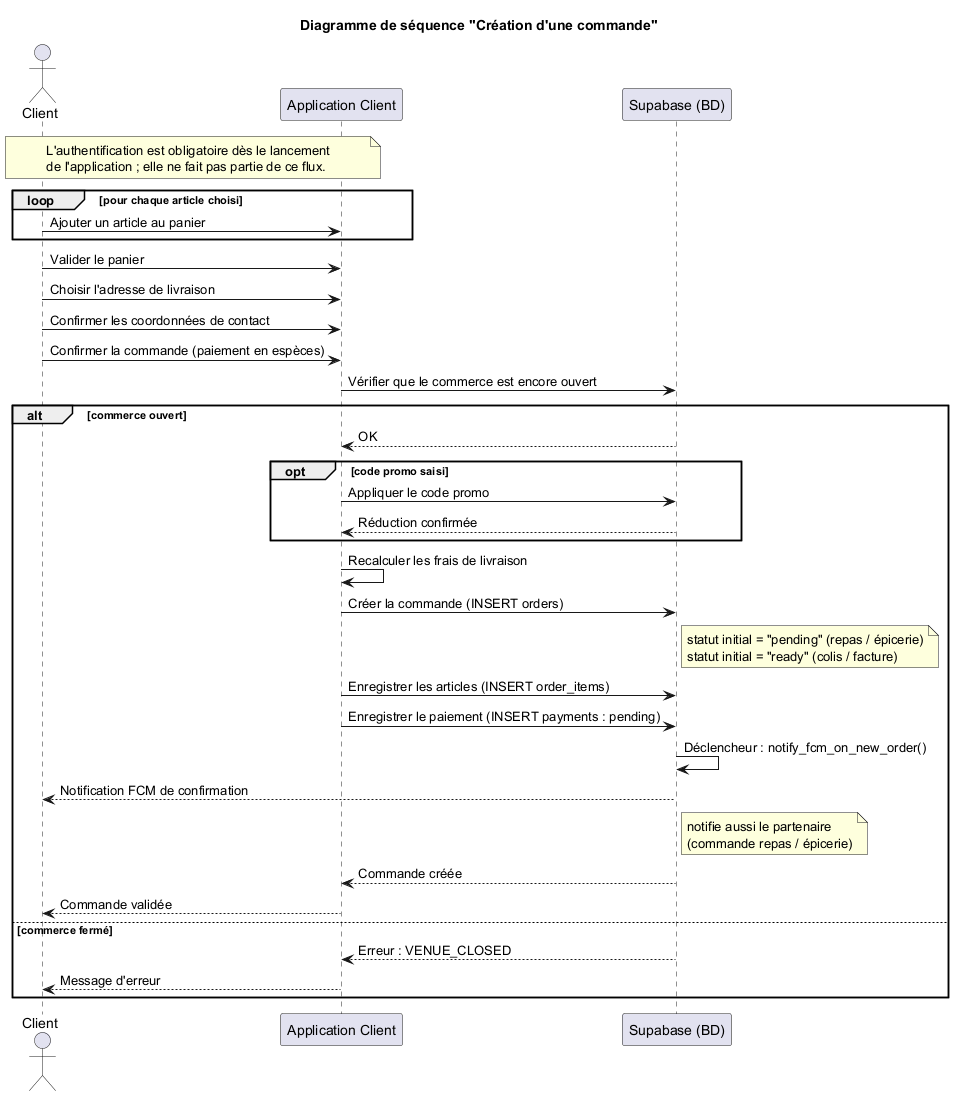
\includegraphics[width=\textwidth,height=0.85\textheight,keepaspectratio]{diagramme_sequence_creation_commande_v2.png}}
    \caption{Diagramme de séquence "Création d'une commande"}
\end{figure}
\newpage

L'analyse approfondie de ce diagramme de séquence met en exergue une structure de contrôle rigoureuse, articulée autour de mécanismes UML avancés qui garantissent la fiabilité de l'application.

\newpage
\subsection{Livraison d'une commande :}
Le diagramme de séquence dédié à la phase de livraison représente le cœur opérationnel de notre solution technologique.

\begin{figure}[H]
    \centering
    \fbox{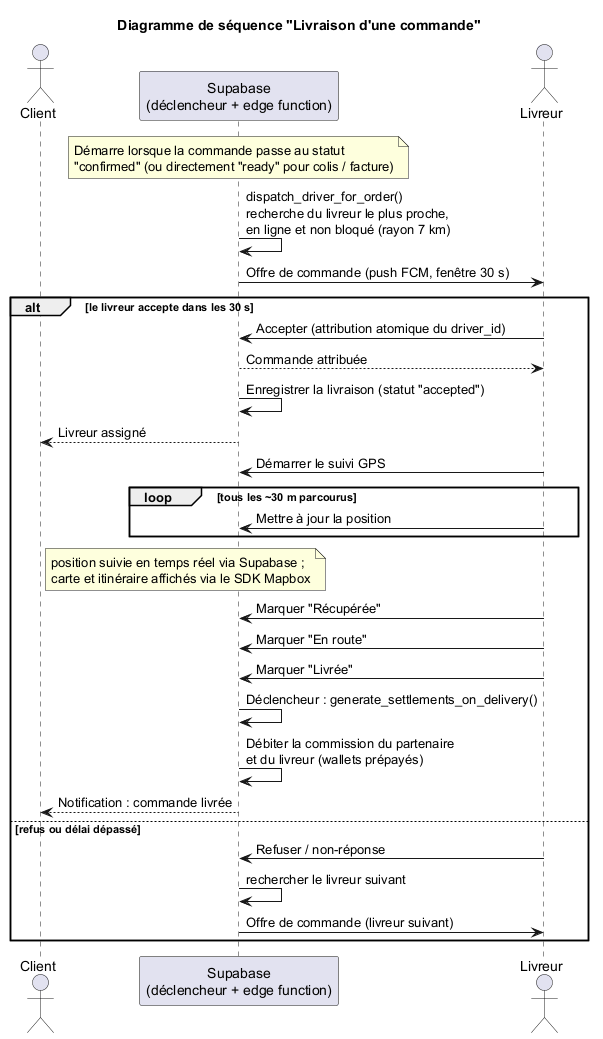
\includegraphics[width=\textwidth,height=0.85\textheight,keepaspectratio]{diagramme_sequence_livraison_commande_v2.png}}
    \caption{Diagramme de séquence "Livraison d'une commande"}
\end{figure}
\newpage

\subsection{Ajout plat du jour :}
Le diagramme de séquence présenté dans cette section illustre une fonctionnalité spécifique et essentielle pour les partenaires restaurateurs.

\begin{figure}[H]
    \centering
    \fbox{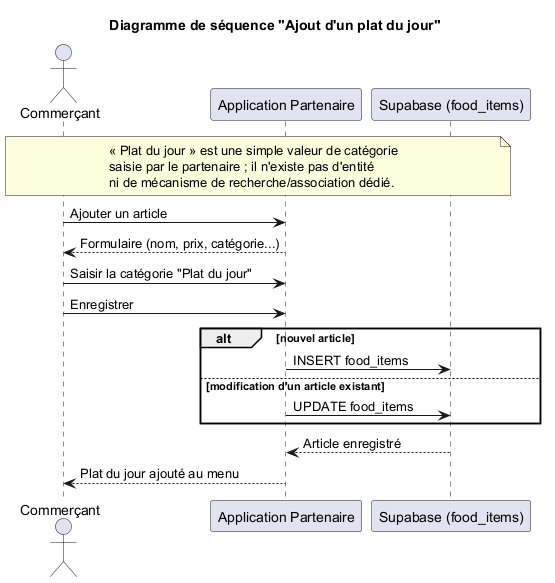
\includegraphics[width=\textwidth,height=0.85\textheight,keepaspectratio]{diagramme_sequence_ajout_plat_jour_v2.png}}
    \caption{Diagramme de séquence "Ajout plat du jour"}
\end{figure}
\newpage


%************CHAP3***********
\chapter{Réalisation et mise en œuvre}

\section{Introduction}

Après la phase d'analyse et de conception, il faut maintenant construire l'application. Ce chapitre explique comment le projet a été réalisé concrètement : les outils utilisés, les technologies choisies, la façon dont le code est organisé, puis chacune des quatre applications qui composent la plateforme Amana, avec leurs fonctionnalités et leurs interfaces principales.

\section{Environnement de développement}

Le développement a été fait avec Visual Studio Code et Android Studio, en utilisant le SDK Flutter (version 3.0 ou plus récente) et le langage Dart (version 3.0). L'application Administrateur a été développée séparément, toujours avec Visual Studio Code, mais avec Next.js et TypeScript plutôt qu'avec Flutter.

\section{Technologies utilisées}

\subsection{Technologies front-end}

Trois des quatre applications du projet — Client, Livreur et Partenaire — partagent le même socle technique : Flutter et le langage Dart. Ce choix permet d'écrire un seul code source pour Android et iOS, avec la même apparence sur les deux systèmes, et de réutiliser une partie du code d'une application à l'autre.

L'application Administrateur suit une logique différente : ce n'est pas une application mobile, mais un tableau de bord web. Elle est construite avec Next.js (un framework basé sur React) et TypeScript, avec Tailwind CSS pour la mise en forme. Ce choix est logique : un administrateur travaille depuis un ordinateur, pas depuis un téléphone, donc une interface web est plus adaptée à son usage.

\subsection{Technologies back-end}

Supabase a été utilisé comme solution back-end pour les quatre applications. Cette plateforme regroupe plusieurs services utiles : une base de données PostgreSQL, un système d'authentification, un mécanisme de mise à jour en temps réel (Realtime), un espace de stockage pour les fichiers (photos de plats, photos de colis, logos), et un environnement pour exécuter des fonctions côté serveur (Edge Functions). Ces fonctions serveur servent aussi bien aux deux fonctionnalités d'intelligence artificielle présentées dans le chapitre précédent qu'à l'envoi des notifications et à la répartition des commandes entre les livreurs.

\section{Architecture du système}

\subsection{Vue d'ensemble}

Le système repose sur une architecture client-serveur. Les trois applications mobiles (Client, Livreur, Partenaire) et le tableau de bord web Administrateur jouent toutes le rôle de couche de présentation : elles ne contiennent pas de logique métier lourde et communiquent directement avec Supabase, qui centralise les données et les règles du système. Chaque application ne voit que les données qui la concernent, grâce aux règles de sécurité définies au niveau des lignes de la base de données (\textit{Row Level Security}).

\subsection{Organisation du code et gestion d'état}

Les trois applications Flutter suivent la même organisation de code, pour rester cohérentes entre elles. Chaque fonctionnalité (commandes, profil, panier, etc.) est rangée dans son propre dossier, séparé en trois parties :

\begin{itemize}
    \item un dossier \texttt{data}, qui contient les modèles de données et un \emph{repository} — une classe qui centralise tous les échanges avec Supabase pour cette fonctionnalité ;
    \item un dossier \texttt{providers}, qui contient la logique métier et l'état de l'application, géré avec la librairie Riverpod ;
    \item un dossier \texttt{presentation}, qui contient les écrans et les widgets, qui affichent simplement les données préparées par les providers.
\end{itemize}

Ce découpage évite de mélanger l'affichage et la logique, sans ajouter de couche supplémentaire de type MVVM : il n'existe pas de classe \emph{ViewModel} séparée dans le projet. C'est directement le \emph{provider} Riverpod qui joue ce rôle intermédiaire entre les données et l'écran. Ce choix garde le code simple à comprendre, tout en restant assez organisé pour qu'un développeur retrouve facilement ses repères d'une application à l'autre. Le tableau de bord Administrateur, lui, n'utilise pas Riverpod puisqu'il n'est pas construit avec Flutter : il gère son état directement avec les outils habituels de React.

\subsection{Modèle de données}

La base de données PostgreSQL est commune aux quatre applications. Elle regroupe toutes les informations du système : comptes utilisateurs, restaurants et supermarchés, produits, commandes, livraisons, portefeuilles et commissions, programme de fidélité, codes promotionnels, etc. Chaque application ne peut lire et modifier que les données qui la concernent, grâce aux règles de sécurité (RLS) définies sur chaque table.

\section{Présentation des applications}

\subsection{Application Client}
\textbf{Utilisateurs cibles :}\\
L'application Client est destinée au grand public : toute personne disposant d'un smartphone Android ou iOS et souhaitant commander un repas, faire ses courses, envoyer un colis ou faire payer une facture.

\vspace{0.3cm}
\textbf{Fonctionnalités principales :}\\
Depuis un écran d'accueil unique, le client choisit entre plusieurs services : commander dans un restaurant, faire ses courses dans un supermarché partenaire, envoyer un colis à une autre personne, ou faire payer une facture par un livreur. Il peut suivre sa commande en temps réel sur une carte, consulter son historique, gérer ses adresses et ses moyens de paiement, cumuler des points dans un programme de fidélité, et poser une question à l'assistant intelligent ou chercher un plat par photo — les deux fonctionnalités présentées en détail dans le chapitre précédent.

\subsection{Application Livreur}
\textbf{Utilisateurs cibles :}\\
Cette application est destinée aux livreurs partenaires de la plateforme, équipés d'un smartphone avec GPS et connexion internet.

\vspace{0.3cm}
\textbf{Fonctionnalités principales :}\\
Le livreur se déclare disponible ou non depuis l'écran d'accueil. Quand il est disponible, il reçoit les commandes proposées et dispose d'un court délai pour les accepter ou les refuser. Une fois une commande acceptée, l'application affiche l'itinéraire à suivre sur une carte, envoie sa position en continu, et lui permet de mettre à jour le statut de la livraison étape par étape, jusqu'à la remise finale. Le livreur peut aussi consulter ses revenus et son solde de portefeuille.

\subsection{Application Partenaire}
\textbf{Utilisateurs cibles :}\\
Cette application est destinée aux restaurateurs, aux responsables de supermarchés et, plus largement, à tous les commerçants partenaires qui gèrent leurs commandes via la plateforme.

\vspace{0.3cm}
\textbf{Fonctionnalités principales :}\\
Le commerçant gère son catalogue de produits (ajout, modification, disponibilité, horaires d'ouverture) et reçoit les nouvelles commandes en direct, avec une alerte sonore. Il peut les accepter ou les refuser, suivre leur préparation, et consulter ses statistiques du jour (chiffre d'affaires, nombre de commandes) ainsi que son solde de portefeuille et les commissions prélevées par la plateforme.

\subsection{Application Administrateur}
\textbf{Utilisateurs cibles :}\\
Cette application est destinée à l'équipe qui supervise l'ensemble de la plateforme. Contrairement aux trois autres applications, ce n'est pas une application mobile mais un tableau de bord web, pensé pour être utilisé depuis un ordinateur.

\vspace{0.3cm}
\textbf{Fonctionnalités principales :}\\
Le tableau de bord donne une vue d'ensemble de l'activité du jour : commandes, livreurs en ligne, restaurants actifs, commissions, revenu total. Il permet de gérer les clients, les restaurants et supermarchés partenaires, les livreurs (y compris leur position en direct), les commandes en cours, les finances sous forme de graphiques, le programme de fidélité et les codes promotionnels, ainsi que les paramètres du système comme les taux de commission. Un journal d'activité garde une trace de toutes les actions sensibles effectuées par les administrateurs, comme le blocage d'un compte.

\section{Interfaces des applications}

Cette section présente les principales interfaces des quatre applications. Chaque figure ci-dessous représente un emplacement prévu pour une capture d'écran réelle de l'application.

\subsection{Interfaces de l'application Client}

\begin{figure}[H]
    \centering
    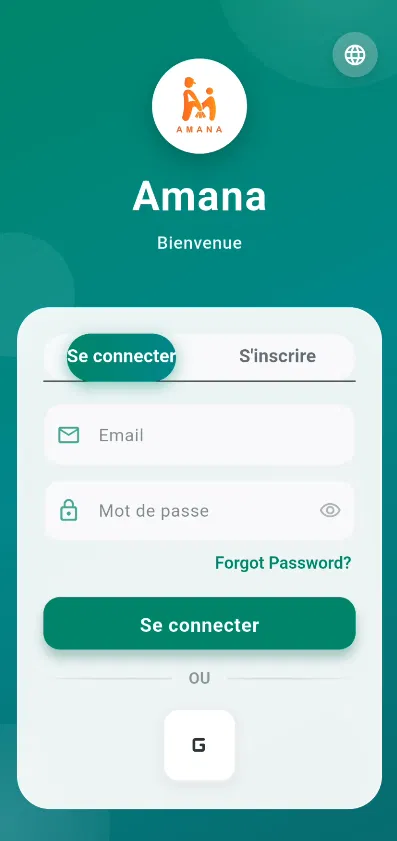
\includegraphics[height=0.5\textheight,keepaspectratio]{images/client_auth.png}
    \caption{Écran d'authentification — application Client}
\end{figure}

\begin{figure}[H]
    \centering
    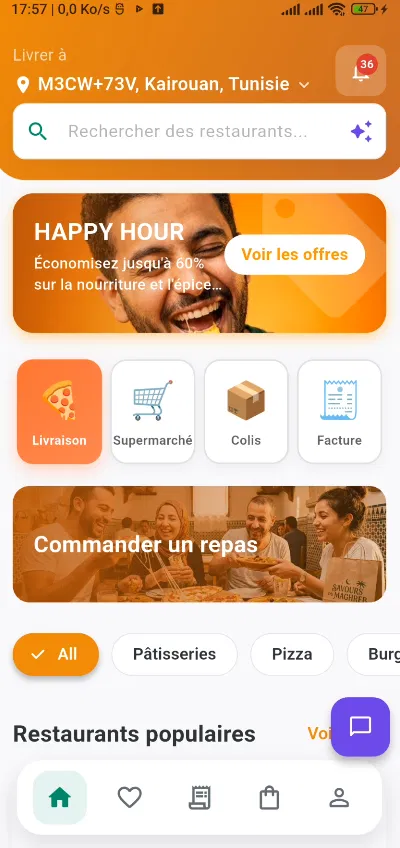
\includegraphics[height=0.5\textheight,keepaspectratio]{images/client_accueil.png}
    \caption{Écran d'accueil — application Client}
\end{figure}

\begin{figure}[H]
    \centering
    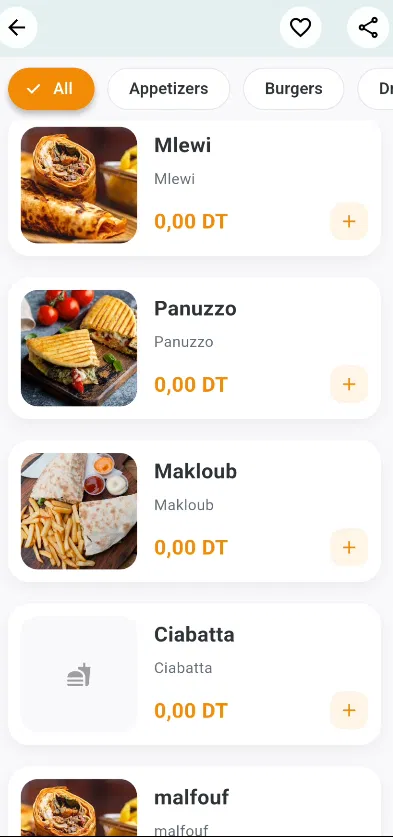
\includegraphics[height=0.5\textheight,keepaspectratio]{images/client_restaurant_detail.png}
    \caption{Détail d'un restaurant et de son menu — application Client}
\end{figure}

\begin{figure}[H]
    \centering
    \includegraphics[height=0.5\textheight,keepaspectratio]{images/client_panier.png}
    \caption{Panier — application Client}
\end{figure}

\begin{figure}[H]
    \centering
    \includegraphics[height=0.5\textheight,keepaspectratio]{images/client_checkout.png}
    \caption{Validation de la commande — application Client}
\end{figure}

\begin{figure}[H]
    \centering
    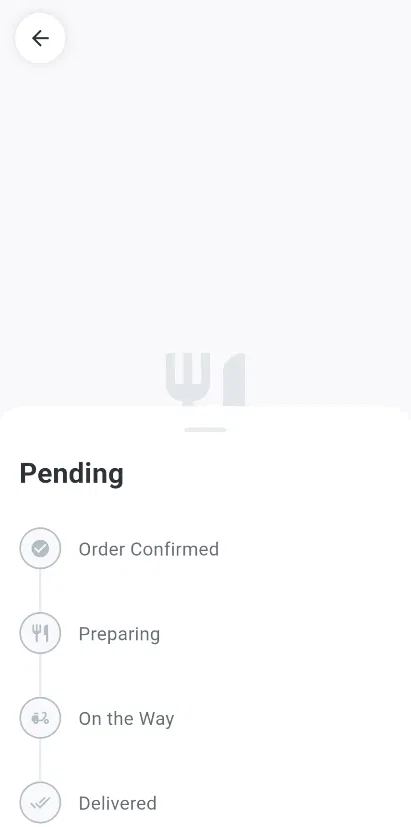
\includegraphics[height=0.5\textheight,keepaspectratio]{images/client_suivi_commande.png}
    \caption{Suivi de la commande en temps réel — application Client}
\end{figure}

\begin{figure}[H]
    \centering
    
\includegraphics[height=0.5\textheight,keepaspectratio]{images/client_assistant_ia.png}
    \caption{Assistant conversationnel — application Client}
\end{figure}

\begin{figure}[H]
    \centering
    
\includegraphics[height=0.5\textheight,keepaspectratio]{images/client_recherche_ia.png}
    \caption{Recherche intelligente — application Client}
\end{figure}

\subsection{Interfaces de l'application Livreur}

\begin{figure}[H]
    \centering
    \includegraphics[height=0.5\textheight,keepaspectratio]{images/livreur_auth.png}
    \caption{Écran d'authentification — application Livreur}
\end{figure}

\begin{figure}[H]
    \centering
    \includegraphics[height=0.5\textheight,keepaspectratio]{images/livreur_accueil.png}
    \caption{Tableau de bord et statut en ligne — application Livreur}
\end{figure}

\begin{figure}[H]
    \centering
    \includegraphics[height=0.5\textheight,keepaspectratio]{images/livreur_commandes_disponibles.png}
    \caption{Liste des commandes disponibles — application Livreur}
\end{figure}

\begin{figure}[H]
    \centering
    \includegraphics[height=0.5\textheight,keepaspectratio]{images/livreur_offre_commande.png}
    \caption{Offre de commande à accepter ou refuser — application Livreur}
\end{figure}

\begin{figure}[H]
    \centering
    \includegraphics[height=0.5\textheight,keepaspectratio]{images/livreur_suivi_livraison.png}
    \caption{Suivi de la livraison en cours — application Livreur}
\end{figure}

\begin{figure}[H]
    \centering
    \includegraphics[height=0.5\textheight,keepaspectratio]{images/livreur_revenus.png}
    \caption{Revenus et portefeuille — application Livreur}
\end{figure}

\subsection{Interfaces de l'application Partenaire}

\begin{figure}[H]
    \centering
    \includegraphics[height=0.5\textheight,keepaspectratio]{images/partenaire_auth.png}
    \caption{Écran d'authentification — application Partenaire}
\end{figure}

\begin{figure}[H]
    \centering
    \includegraphics[height=0.5\textheight,keepaspectratio]{images/partenaire_accueil.png}
    \caption{Tableau de bord du commerçant — application Partenaire}
\end{figure}

\begin{figure}[H]
    \centering
    \includegraphics[height=0.5\textheight,keepaspectratio]{images/partenaire_menu.png}
    \caption{Catalogue de produits — application Partenaire}
\end{figure}

\begin{figure}[H]
    \centering
    \includegraphics[height=0.5\textheight,keepaspectratio]{images/partenaire_ajout_article.png}
    \caption{Ajout / modification d'un article — application Partenaire}
\end{figure}

\begin{figure}[H]
    \centering
    \includegraphics[height=0.5\textheight,keepaspectratio]{images/partenaire_commande_entrante.png}
    \caption{Nouvelle commande entrante — application Partenaire}
\end{figure}

\begin{figure}[H]
    \centering
    \includegraphics[height=0.5\textheight,keepaspectratio]{images/partenaire_liste_commandes.png}
    \caption{Liste des commandes — application Partenaire}
\end{figure}

\begin{figure}[H]
    \centering
    \includegraphics[height=0.5\textheight,keepaspectratio]{images/partenaire_portefeuille.png}
    \caption{Portefeuille et commissions — application Partenaire}
\end{figure}

\subsection{Interfaces de l'application Administrateur}

\begin{figure}[H]
    \centering
    \includegraphics[width=0.85\textwidth,keepaspectratio]{images/admin_login.png}
    \caption{Écran de connexion — tableau de bord Administrateur}
\end{figure}

\begin{figure}[H]
    \centering
    \includegraphics[width=0.85\textwidth,keepaspectratio]{images/admin_dashboard.png}
    \caption{Vue d'ensemble — tableau de bord Administrateur}
\end{figure}

\begin{figure}[H]
    \centering
    \includegraphics[width=0.85\textwidth,keepaspectratio]{images/admin_commandes.png}
    \caption{Gestion des commandes — tableau de bord Administrateur}
\end{figure}

\begin{figure}[H]
    \centering
    \includegraphics[width=0.85\textwidth,keepaspectratio]{images/admin_restaurants.png}
    \caption{Gestion des restaurants et partenaires — tableau de bord Administrateur}
\end{figure}

\begin{figure}[H]
    \centering
    \includegraphics[width=0.85\textwidth,keepaspectratio]{images/admin_livreurs.png}
    \caption{Gestion des livreurs — tableau de bord Administrateur}
\end{figure}

\begin{figure}[H]
    \centering
    \includegraphics[width=0.85\textwidth,keepaspectratio]{images/admin_finances.png}
    \caption{Finances — tableau de bord Administrateur}
\end{figure}

\begin{figure}[H]
    \centering
    \includegraphics[width=0.85\textwidth,keepaspectratio]{images/admin_parametres.png}
    \caption{Paramètres du système — tableau de bord Administrateur}
\end{figure}

\section{Conclusion}

Ce chapitre a présenté la réalisation concrète de la plateforme Amana : les technologies choisies, l'organisation du code, l'architecture générale, ainsi que les quatre applications qui composent le système, avec leurs fonctionnalités et leurs interfaces principales. On retrouve une cohérence forte entre les trois applications mobiles, qui partagent la même base technique et la même organisation de code, et une application Administrateur pensée différemment, comme un outil web de supervision destiné à un usage depuis un ordinateur plutôt qu'un téléphone. Cette réalisation reprend fidèlement les choix faits dans les chapitres précédents, tout en les adaptant aux contraintes réelles du développement.

\end{justify}
\end{document}
